\documentclass[german,oneside]{thesisclass}
% Based on thesisclass.cls of Timo Rohrberg, 2009
% ----------------------------------------------------------------
% Thesis - Main document
% ----------------------------------------------------------------


%% -------------------------------
%% |  Information for PDF file   |
%% -------------------------------
\hypersetup{
 pdfauthor={Wolfgang Heni, Sebastian Heunisch},
 pdftitle={Labor Nanotechnologie - Direct Laser Writing und Raster Elektronenmikroskopie},
 pdfsubject={},
 pdfkeywords={OLED}
}


%% ---------------------------------
%% | Information about the thesis  |
%% ---------------------------------

\newcommand{\myname}{Wolfgang Heni \\ Sebastian Heunisch}
\newcommand{\mytitle}{Direct Laser Writing und Raster Elektronenmikroskopie}
\newcommand{\myinstitute}{Lichttechnisches Institut (LTI)}

\newcommand{\reviewerone}{?}
\newcommand{\reviewertwo}{?}
\newcommand{\advisor}{Carsten Eschenbaum (M.Eng.)}
\newcommand{\advisortwo}{?}

\newcommand{\timestart}{24. Januar 2011}
\newcommand{\timeend}{XX. Monat 20XX}
\newcommand{\submissiontime}{DD. MM. 20XX}


%% ---------------------------------
%% | ToDo Marker - only for draft! |
%% ---------------------------------
% Remove this section for final version!
\setlength{\marginparwidth}{20mm}

\newcommand{\margtodo}
{\marginpar{\textbf{\textcolor{red}{ToDo}}}{}}

\newcommand{\todo}[1]
{{\textbf{\textcolor{red}{(\margtodo{}#1)}}}{}}


%% --------------------------------
%% | Old Marker - only for draft! |
%% --------------------------------
% Remove this section for final version!
\newenvironment{deprecated}
{\begin{color}{gray}}
{\end{color}}


%% --------------------------------
%% | Settings for word separation |
%% --------------------------------
% Help for separation:
% In german package the following hints are additionally available:
% "- = Additional separation
% "| = Suppress ligation and possible separation (e.g. Schaf"|fell)
% "~ = Hyphenation without separation (e.g. bergauf und "~ab)
% "= = Hyphenation with separation before and after
% "" = Separation without a hyphenation (e.g. und/""oder)

% Describe separation hints here:
\hyphenation{
% Pro-to-koll-in-stan-zen
% Ma-na-ge-ment  Netz-werk-ele-men-ten
% Netz-werk Netz-werk-re-ser-vie-rung
% Netz-werk-adap-ter Fein-ju-stier-ung
% Da-ten-strom-spe-zi-fi-ka-tion Pa-ket-rumpf
% Kon-troll-in-stanz
}


%% ------------------------
%% |    Including files   |
%% ------------------------
% Only files listed here will be included!
% Userful command for partially translating the document (for bug-fixing e.g.)
\includeonly{%
titlepage,
introduction,
content,
appendix
}


%%%%%%%%%%%%%%%%%%%%%%%%%%%%%%%%%
%% Here, main documents begins %%
%%%%%%%%%%%%%%%%%%%%%%%%%%%%%%%%%
\begin{document}

% Remove the following line for German text
%\selectlanguage{english}

\frontmatter
\pagenumbering{roman}
%% titlepage.tex
%%

% coordinates for the bg shape on the titlepage
\newcommand{\diameter}{20}
\newcommand{\xone}{-15}
\newcommand{\xtwo}{160}
\newcommand{\yone}{15}
\newcommand{\ytwo}{-253}

\begin{titlepage}
% bg shape
\begin{tikzpicture}[overlay]
\draw[color=gray]  
 		 (\xone mm, \yone mm)
  -- (\xtwo mm, \yone mm)
 arc (90:0:\diameter pt) 
  -- (\xtwo mm + \diameter pt , \ytwo mm)
	-- (\xone mm + \diameter pt , \ytwo mm)
 arc (270:180:\diameter pt)
	-- (\xone mm, \yone mm);
\end{tikzpicture}
	\begin{textblock}{10}[0,0](4,2.5)
		
\includegraphics[width=.3\textwidth]{logos/KITLogo_RGB.pdf}
	\end{textblock}
	\changefont{phv}{m}{n}	% helvetica	
	\vspace*{2cm}
	\begin{center}
		\huge{\mytitle}
		\vspace*{2cm}\\
		\Large{
			\iflanguage{english}{Diploma Thesis of}			
												  {Laborbericht\\von}
		}\\
		\vspace*{1cm}
		\huge{\myname}\\
		\vspace*{1cm}
		\Large{
			\iflanguage{english}{At the faculty of Computer Science}			
													{An der Fakult\"at f�r Elektro- und Informationstechnik}
			\\
			\myinstitute
		}
	\end{center}
	\vspace*{1cm}
\Large{
\begin{center}
\begin{tabular}[ht]{l c l}
%  \iflanguage{english}{Reviewer}{Erstgutachter}: & \hfill  & \reviewerone\\
%  \iflanguage{english}{Second reviewer}{Zweitgutachter}: & \hfill  & \reviewertwo\\
  \iflanguage{english}{Advisor}{Betreuer}: & \hfill  & \advisor\\
%  \iflanguage{english}{Second advisor}{Zweiter betreuender Mitarbeiter}: & \hfill  & \advisortwo\\
\end{tabular}
\end{center}
}


\vspace{2cm}
\begin{center}
\large{\iflanguage{english}{Time (?)}{} \timestart \hspace*{0.25cm}}
\end{center}


\begin{textblock}{10}[0,0](4,16.8)
\tiny{ 
	\iflanguage{english}
		{KIT -- University of the State of Baden-Wuerttemberg and National Laboratory of the Helmholtz Association}
		{KIT -- Universit�t des Landes Baden-W�rttemberg und nationales Forschungszentrum der Helmholtz-Gesellschaft}
}
\end{textblock}

\begin{textblock}{10}[0,0](14,16.75)
\large{
	\textbf{www.kit.edu} 
}
\end{textblock}

\end{titlepage}

\blankpage


%% -------------------
%% |   Directories   |
%% -------------------
\tableofcontents
\blankpage


%% -----------------
%% |   Main part   |
%% -----------------
\mainmatter
\pagenumbering{arabic}
%% introduction.tex
%%

%% ==============================
\chapter{Einleitung}
\label{ch:Introduction}
%% ==============================
Die Strukturierung von Werkstoffen ist ein Problem, das die Menschheit schon seit Jahrtausenden besch"aftigt. Schon in der Steinzeit haben sich die Menschen damit beschtigt, wie man aus harten Steinen Werkzeuge formen kann, die das Leben im Alltag erleichtern. Auch in der Mikroelektronik spielt die Strukturierung eine wichtige Rolle. Durch die Miniaturisierung werden die Herstellungskosten gesenkt und es lassen sich schnellere und spaarsamere integrierte Schaltungen produzieren. Das in der Mikroelektronik am h"aufigsten verwendete Strukturierungsverfahren ist die optische Lithographie. Diese erm"oglicht eine schnelle kosteng"unstige Strukturierung mit einer Aufl"osung kleiner 100~nm. F"ur bestimmte Anwendungen ist es jedoch notwendig dreidimensionale Strukturen zu schreiben.

Ein Strukturierungsverfahren das die Herstellung dreidimensionaler Strukturen erm�glicht ist das \textit{Direct Laser Writing} (DLW). Um die geschriebenen Strukturen zu charakterisieren kann ein Raster Elektronen Mikropskop (REM) genutzt werden.

Mit Hilfe eines REMs ist es m�glich, Strukturen im Mikro- und Nanometerbereich aufzul�sen und zu betrachten. Daher ist es ein Standardwerkzeug in vielen wissenschaftlichen Arbeitsfeldern.  Sowohl das Schreiben von Strukturen mit DLW als auch die Charakterisierung mittels eines REMs werden am Lichttechnischen Institut am Karlsruher Institut f�r Technologie durchgef�hrt. 

Im Versuch "`Direct Laser Writing und Raster Elektronenmikroskopie"' des Labors Nanoelektronik am Lichttechnischen Institut  wird daher ein  Einblick in das Arbeiten mit dem Raster Elektronen Mikroskop und das Herstellen dreidimensionaler Strukturen im Mikrometerbereich mit \textit{Direct Laser Writing} gegeben. 

%Ein m"ogliches neues Strukturierungsverfahren, das ebenfalls Strukturgr"osen mit hoher Aufl"osung erm"oglicht, ist die Laserinterferenzlithografie. 

%  Bis Heute haben sich zwar die verwendeten Materialien ge"andert, es sind jedoch immernoch Leistungsf"ahige Strukturierungsverfahren f"ur diese Materialien erforderlich. Auch die Anforderungen an die Materialien haben sich ge"andert. In der Mikroelektronik  
% 
%  als \todo{ich wills jetzt net zu arg breittreten. ma k"onnt noch was "uber die Strukturierung von anderen Materialien erz"ahlen: Metall gie"sen - schmieden - usw}.
% Auch in der Neuzeit besch"aftigen sich zahlreiche Wissenschaftler und Ingineure damit wie man Werkstoffe strukturieren kann. F"ur 
%% content.tex
%%

%% ==============
\chapter{Grundlagen}
\label{ch:Grundlagen}
%% ==============
\section{Rasterelektronenmikroskop}
\label{ch:Grundlagen:sec:REM}


\begin{figure}[h]%
\centering
%\begin{adjustwidth}{-1.5cm}{0cm}
	\subfloat[Zonen der Elektronenemission \cite{MNO}.]{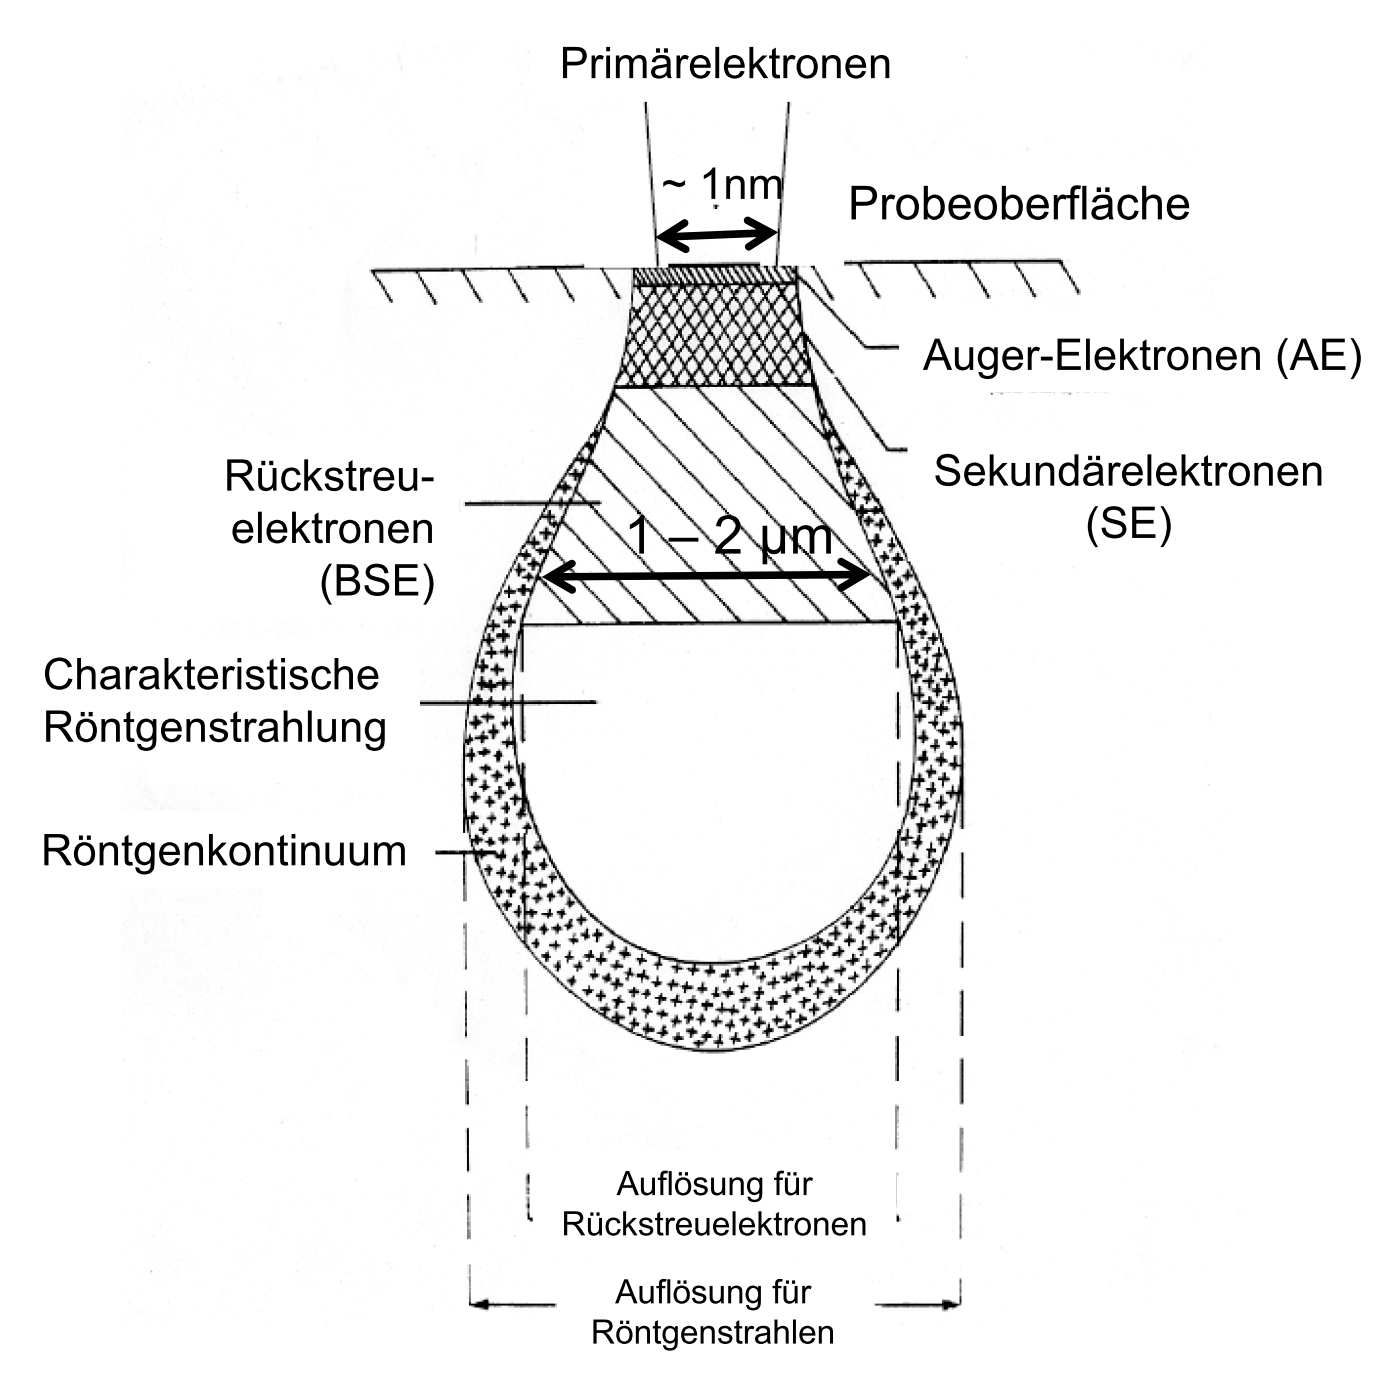
\includegraphics[width=.5\columnwidth]{Grafiken/ionisationsbirne.jpg}\label{fig:ionisationsbirne}}
	\subfloat[Schematischer Aufbau eines REMs \cite{Colliex}.]{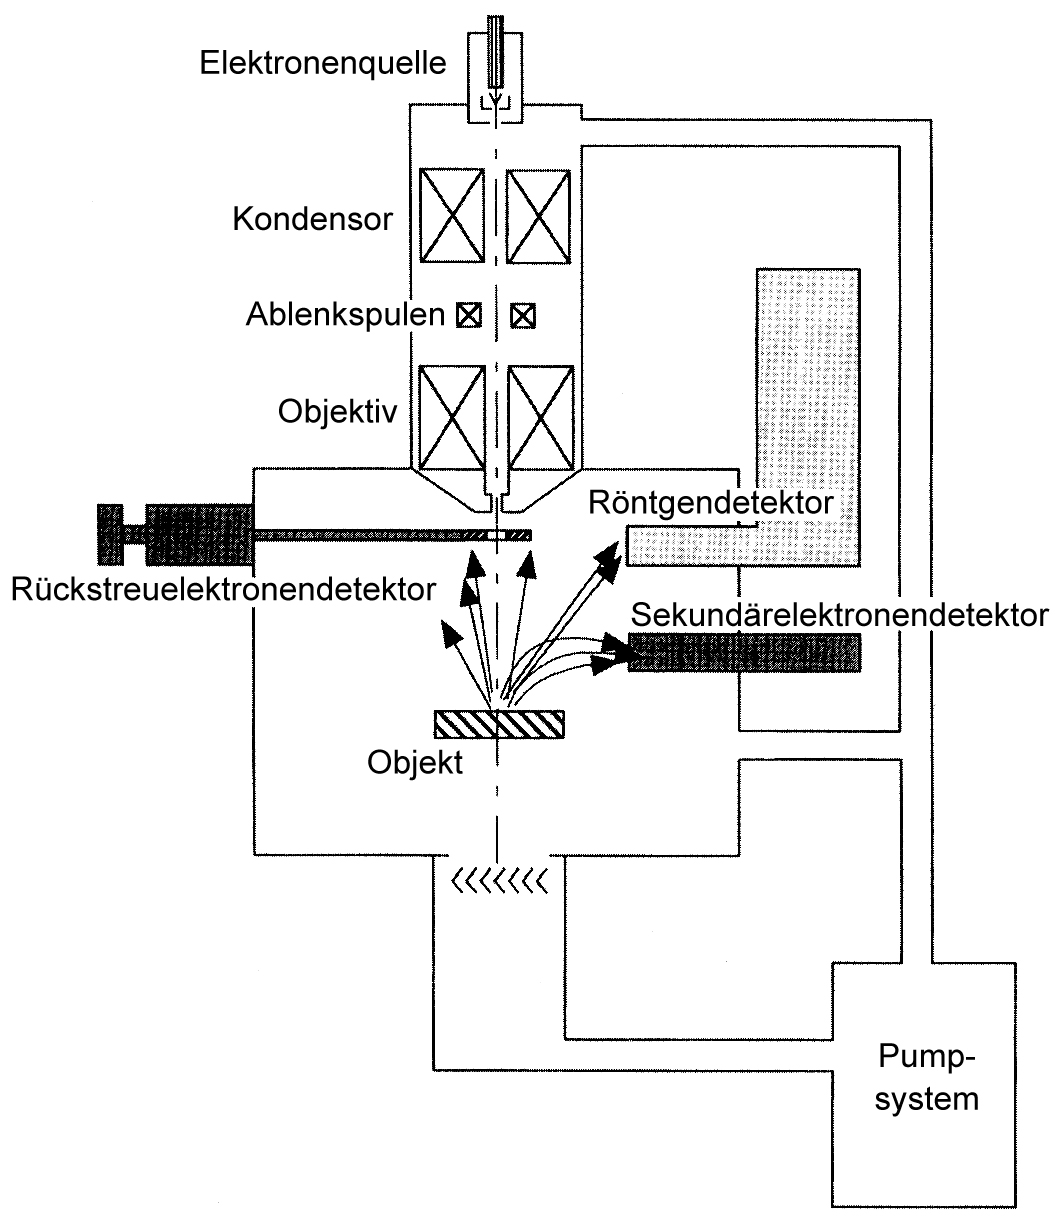
\includegraphics[width=.5\columnwidth]{Grafiken/rem-schema-1.jpg} \label{fig:aufbau_rem}}%
%	\end{adjustwidth}
\caption{}%
\label{fig:rem_subfig}%
\end{figure}
Mit einem Rasterelektronenmikroskop k�nnen durch die Wechselwirkung eines Elektronenstrahls mit dem Material einer zu betrachtenden Probe hochaufl�sende Bilder dieser Probe angefertigt werden.

In Abbildung \ref{fig:aufbau_rem} ist schematisch der Aufbau eines Ras\-ter\-elektro\-nen\-mikros\-kops (REM) dargestellt. Aus einer Elektronenquelle werden durch eine Spannung $U_{B}$ von einigen kV Elektronen (Prim"ar Elektronen - PE) aus einer Kathode gel"ost und beschleunigt. Durch ein System aus Magnetlinsen, Ablenkspulen und Blenden wird ein Elektronenstrahl geformt, mit dem die Probe abgetastet werden kann. Der Aufbau befindet sich in einem evakuierten Geh"au"se, um ein ablenken des Elektronenstrahls durch Luftmolek"ule zu vermeiden. 

Treffen PE auf die Probe werden diese durch elastische oder inelastische Streuung abgebremst. Hierdurch werden von der Probe durch verschiedene Prozesse Teilchen emittiert, die sich in ihrer Energie unterscheiden.

% Bei Elektronen mit einer Energie von weniger als 50~eV spricht man von Sekund"arelektronen~(SE). Diese werden durch inelastische St"o"se der PE mit schwach gebunden Elektronen im Material erzeugt. Seitlich der Probe ist ein Everhart-Thornley-Detektor angebracht. Dieser beschleunigt durch eine Spannung die SE auf einen Szintilationskristall. Trifft ein Elektron auf diesen Kristall sendet er einen Lichtpuls aus, der anschlie"send durch einen Photomultiplier verst"arkt wird und in einen Spannungsimpuls umgewandelt werden.

Bei emittierten Elektronen mit einer Energie von weniger als 50~eV spricht man von Sekund"arelektronen~(SE). Diese werden durch inelastische St"o"se der PE mit schwach gebunden Elektronen im Material erzeugt. Seitlich der Probe ist ein Everhart-Thornley-Detektor angebracht. Dieser zieht durch eine Spannung die SE an. Treffen diese auf den Szintilationskristall des Detektors sendet dieser einen Lichtpuls aus, der anschlie"send durch einen Photomultiplier verst"arkt und in einen Spannungsimpuls umgewandelt wird. Es k"onnen nur SE detektiert werden, die im oberfl"achennahen Bereich des Materials erzeugt wurden (vgl. Abbildung \ref{fig:ionisationsbirne}), da die Energie der SE nicht ausreicht, um aus tieferen Materialschichten nach au"sen zu dringen. Mit SE kann daher die Topografie des Materials mit hoher Aufl"osung vermessen werden.


Elektronen die Tiefer in das Material eindringen und stark vom Material gestreut werden, werden als R"uckstreuelektronen (engl. \textit{Backscattered Electrons} - BSE) bezeichnet. BSE besitzen eine Energie zwischen 50~eV und $ e \cdot U_{\mathrm{B}}$. Sie werden durch einen Detektor, der "uber der Probe um die Apperturblende angebracht ist, detektiert (vgl. Abbildung \ref{fig:aufbau_rem}). Da die Streuung der Elektronen und damit die Energieverteilung der BSE von der Dichte des Untersuchten Materials abh"angt, lassen sich "uber BSE gut Materialkontraste darstellen. Allerdings ist die Aufl"osung geringer als bei SE.

Durch St��e der Elektronen mit den Atomen der Probe k�nnen diese angeregt werden, d.h. Elektronen werden in einen h�heren Energiezustand angehoben. Wenn diese angeregten Elektronen rekombinieren wird entweder R"ontgenstrahlung emmitiert, oder die freiwerdende Energie wird an ein weiteres atomares Elektron "ubertragen, das als Augerelektron emmittiert wird. Da die emmitierten Elektronen bzw. Photonen diskrete Energien besitzen, l"asst sich mit ihnen das Probenmaterial bestimmen \cite{Reimer}.

Um nun ein Bild aufzunehmen, tastet man die Probe mit dem Elektronenstrahl ab. Die gemessenen Detektorinformatioen werden  entweder auf einer Kathodenstrahlr"ohre zeilenweise dargestellt, oder an einen Rechner weitergeleitet und verarbeitet.

% Die Aufl"osung eines Rasterelektronenmikroskops wird durch die Beugung bestimmt. Diese wird durch das Abbe'sche Abbildungskriterium
% \begin{equation}
%  d_{min} \approx \frac{\lambda}{2\cdot NA}
% \label{eq:Abbe}
% \end{equation}
% beschrieben. Wobei $\lambda$ die Wellenl"ange des Teilchens, und $NA$ die Numerische Apperatur der Elektronenoptik bezeichnet. Je h"oher die Enenergie eines Elektrons ist, je n"aher sich das Objekt an der Apperturblende befindet und je weiter die Apperturblende ge"offnet ist, lassen sich also theoretisch kleinere Objekte abbilden \todo{der Satz is komisch}. Jedoch wird die Aufl"osung des Rasterelektronenmikroskops auch durch die Abbildungsfehler des Linsensystems begrenzt. So werden bei Magnetlinsen h"aufig achsferne Strahlen st"arker zur Achse hin gebrochen als achsnahe Strahlen. Daraus resultiert eine starke sph"arische Abberation. Um diesen Abbildungsfehler zu minimieren und somit die Aufl"sung zu erh"ohen, sollte die Apperturblende, anders als in \eqref{eq:Abbe} gezeigt, weiter geschlossen werden.

Die Aufl"osung eines Lichtmikroskops wird durch die Beugung bestimmt. Diese wird durch das Abbe'sche Abbildungskriterium
\begin{equation}
 d_{\mathrm{min}} \approx \frac{\lambda}{2\cdot NA}
\label{eq:Abbe}
\end{equation}
beschrieben. Wobei $\lambda$ die Wellenl"ange der verwendeten Strahlung, und $NA$ die Numerische Apperatur der Optik bezeichnet. Je kleiner also $\lambda$ bzw. je gr"o�er $NA$, desto kleinere Strukturen k"onnen also aufgel"ost werden. Prinzipiell gilt dieser Zusammenhang auch f�r das REM. Dies bedeutet, dass die Elektronenenergie m"oglichst gro"s, die Apperturblende m"oglichst weit ge"offnet und das Objekt m"oglichst nah an der Blende sein muss, um eine hohe Aufl"osung zu erzielen. Die Aufl"osung des Rasterelektronenmikroskops wird jedoch auch stark durch die Abbildungsfehler des Linsensystems begrenzt. So werden bei Magnetlinsen h"aufig achsferne Strahlen st"arker zur Achse hin gebrochen als achsnahe Strahlen. Daraus resultiert eine starke sph"arische Abberation. Um diesen Abbildungsfehler zu minimieren und somit die Aufl"osung zu erh"ohen, sollte die Apperturblende m"oglichst weit geschlossen werden \cite{Reimer}.

In Abbildung \ref{fig:ss} sind Aufnahmen der Augenoberfl�che einer Fliege mit verschiedenen \textit{Spotsize}-Einstellungen dargestellt. Diese wird �ber die Appertur der Elektronenoptik eingestellt. Bei einer Spottsize von 50 (vgl. Abbildung \ref{fig:ss50}) sieht man, dass neben der h�heren sph�rischen Abberation ein weiterer Bildfehler auftritt. Bei gro�er \textit{Spotsize} treffen viele Elektronen auf die Probe, was vor allem bei nichtleitenden Objekten zu einer Aufladung der Probenoberfl�che f�hrt. Hierdurch wird der Elektronenstrahl von der Oberfl�che abgesto�en und das beobachtete Bild verzerrt.

Bei zu geringer Appertur tritt ein weiteres Problem auf. Es treffen nur noch wenige Elektronen auf die Probenoberfl�che, und es werden somit weniger SE generiert. Das detektierte Signal muss stark verst�rkt werden, wodurch sich das Rauschen erh�ht (vgl. Abbildung \ref{fig:ss20}). F�r die betrachteten Proben wurde empirisch eine optimale \textit{Spotsize} von 35 bestimmt (vgl. Abbildung \ref{fig:ss35}).

\begin{figure}%
\centering
\begin{adjustwidth}{-.5cm}{0cm}
	\subfloat[\textit{Spotsize:} 20]{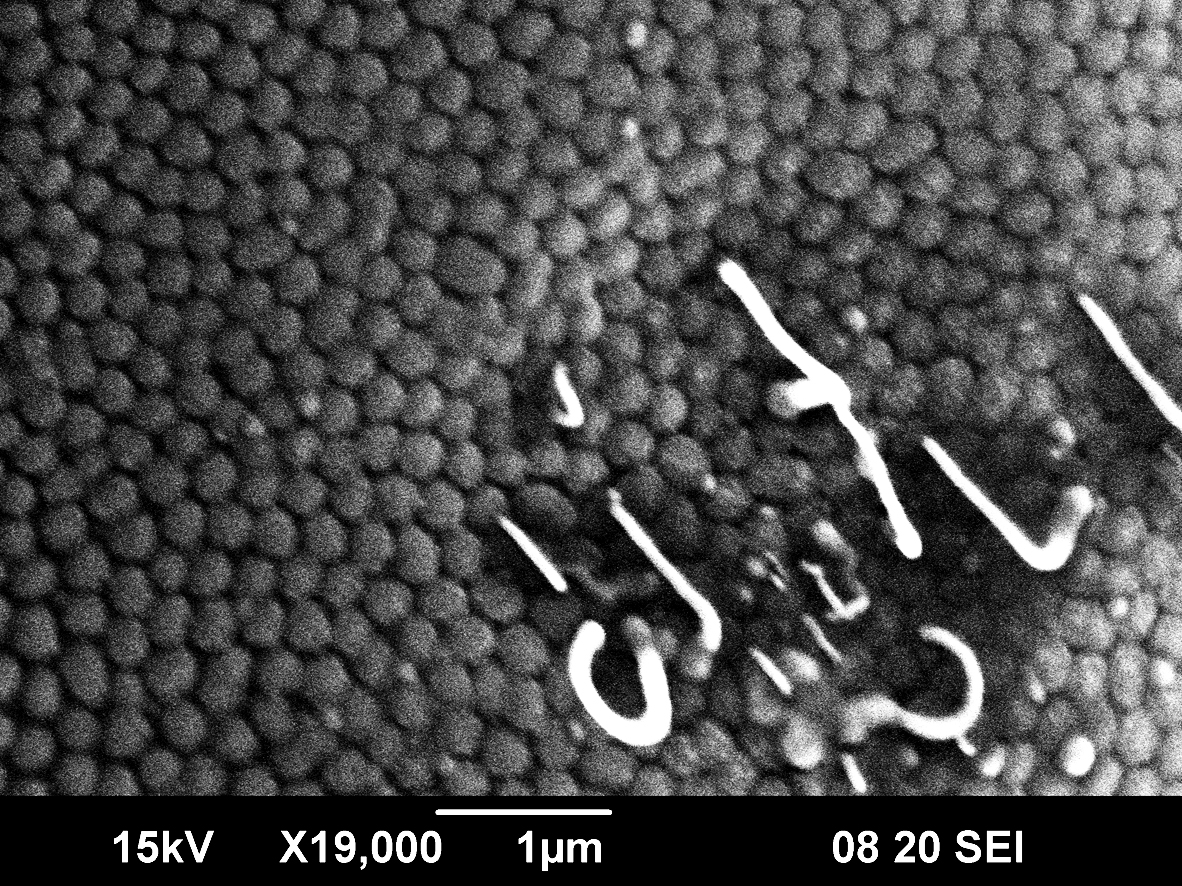
\includegraphics[totalheight=4 cm]{Grafiken/ss20.jpg}\label{fig:ss20}~}
	\subfloat[\textit{Spotsize:} 35]{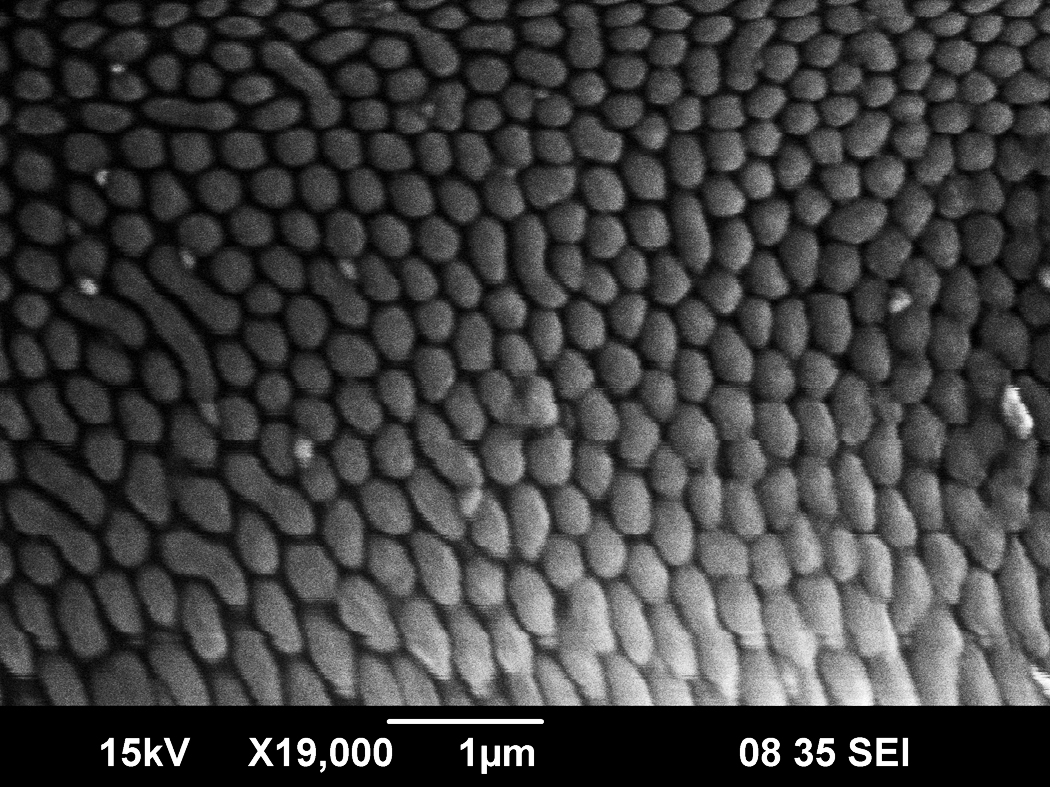
\includegraphics[totalheight=4 cm]{Grafiken/ss35.jpg} \label{fig:ss35}}%
		\subfloat[\textit{Spotsize:} 50]{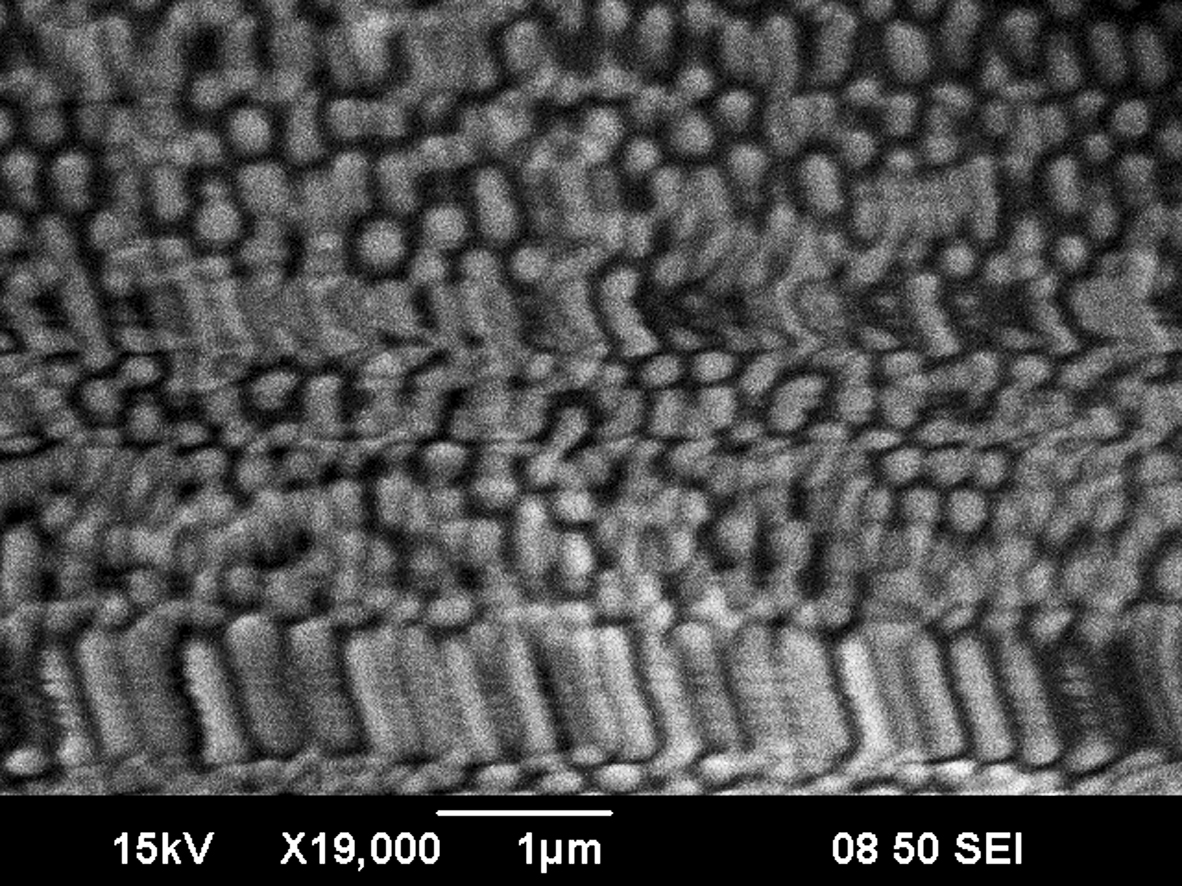
\includegraphics[totalheight=4 cm]{Grafiken/ss50.jpg}\label{fig:ss50}}
\end{adjustwidth}
\caption{SEM-Aufnahmen der Augenoberfl�che einer Fliege mit verschiedenen \textit{Spotsize}-Einstellungen.}%
\label{fig:ss}%
\end{figure}



Ein weiterer Vorteil eines REM gegen"uber einem Lichtmikroskop ist, neben der h"oheren Aufl"osung, die gro"se Tiefensch"arfe. Abbildung \ref{fig:schraube} zeigt eine Aufnahme einer Schraube, zum einen mit dem Lichtmikroskop (a), zum anderen mit dem REM (b). Mit dem Lichtmikroskop (vgl. Abbildung \ref{fig:schraube_licht}) kann nur eine bestimmte Ebene der Schraube fokusiert werden. Man erkennt daher gerade noch eine Windung der Schraube scharf. Durch Messungen mit dem REM wurde dieser Abstand und damit die Tiefensch�rfe des Lichtmikroskops auf ca. 850~$\upmu$m bestimmt. Bei der Rasterelektronenmikroskopie wird die Probe durch einen feinen Strahl abgetastet. Der Bereich der Fokusierung (Raileigh L"ange) ist daher viel gr"o"ser als beim Lichtmikroskop. Daher sind auf Abbildung \ref{fig:schraube_rem} alle Windungen der Schraube zu erkennen.





%
%\begin{figure}
%\centering
%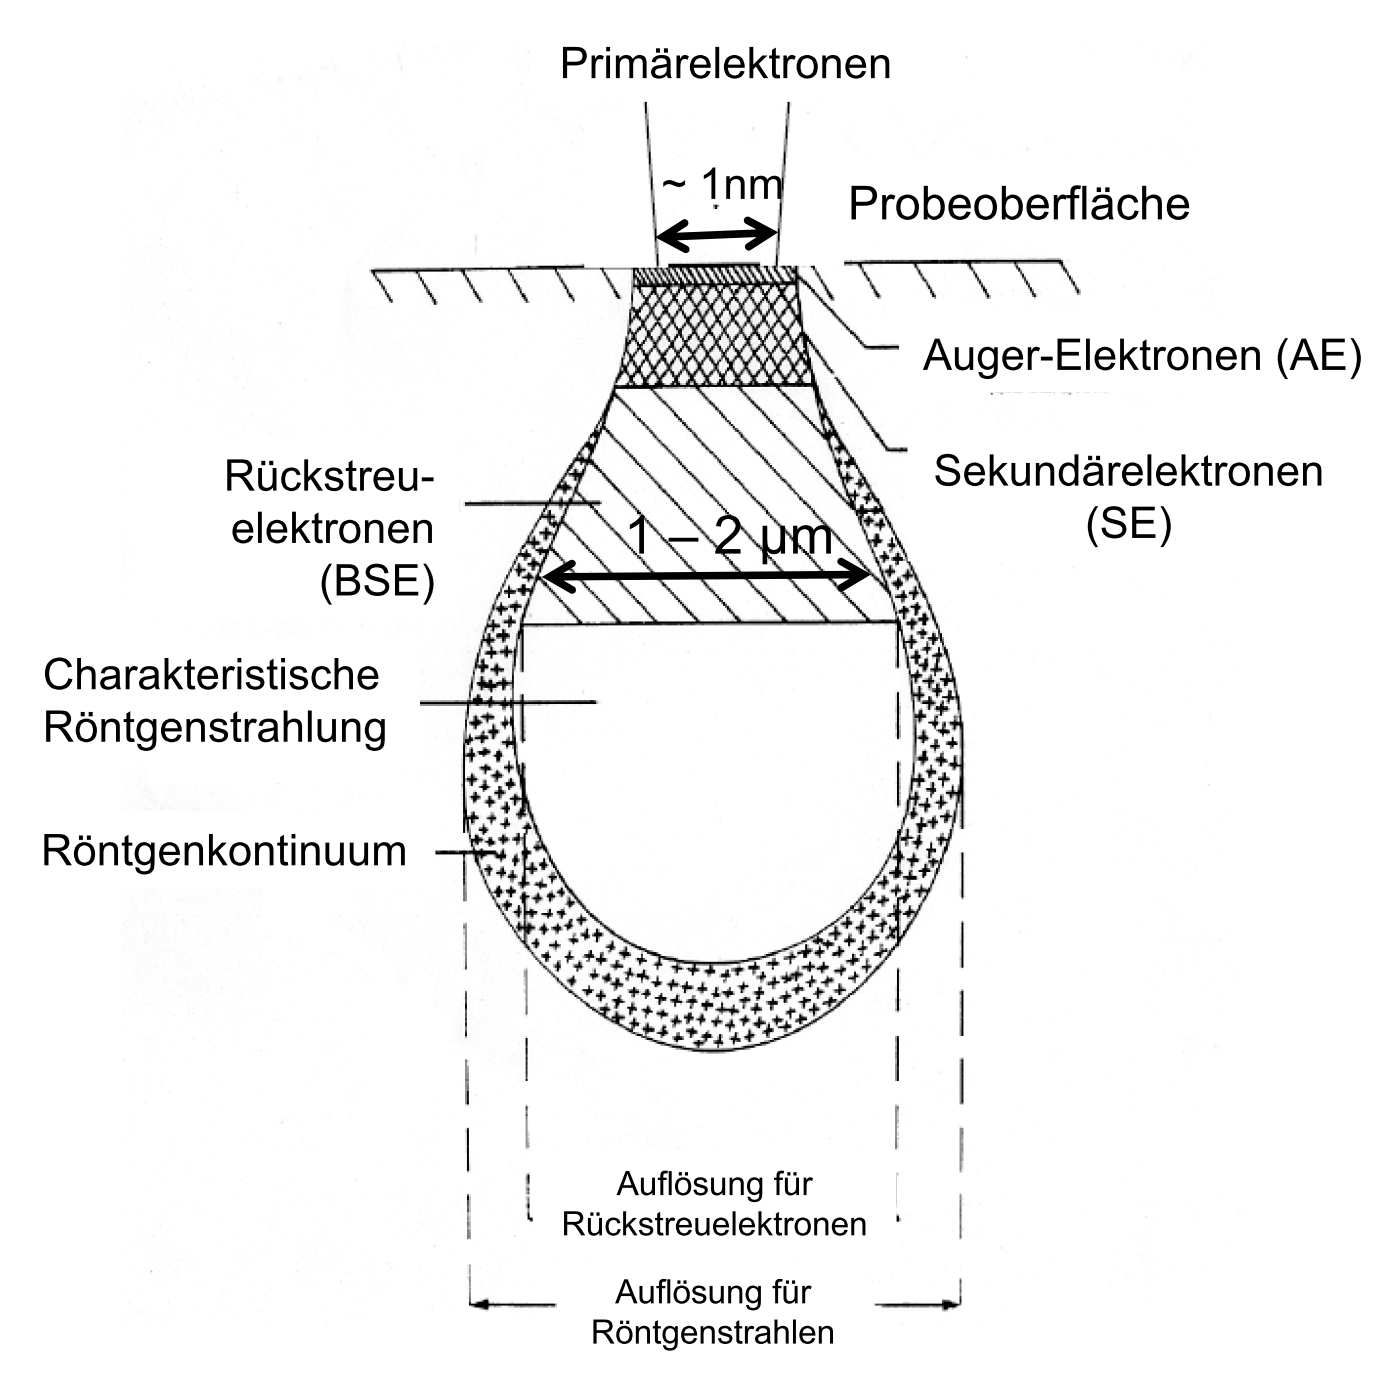
\includegraphics[width=.5\columnwidth]{Grafiken/ionisationsbirne.jpg}%
%\caption{Ionisationsbirne \cite{Reimer}.}
%\label{fig:ionisationsbirne}
%\end{figure} 
%
%\begin{figure}
%\centering
%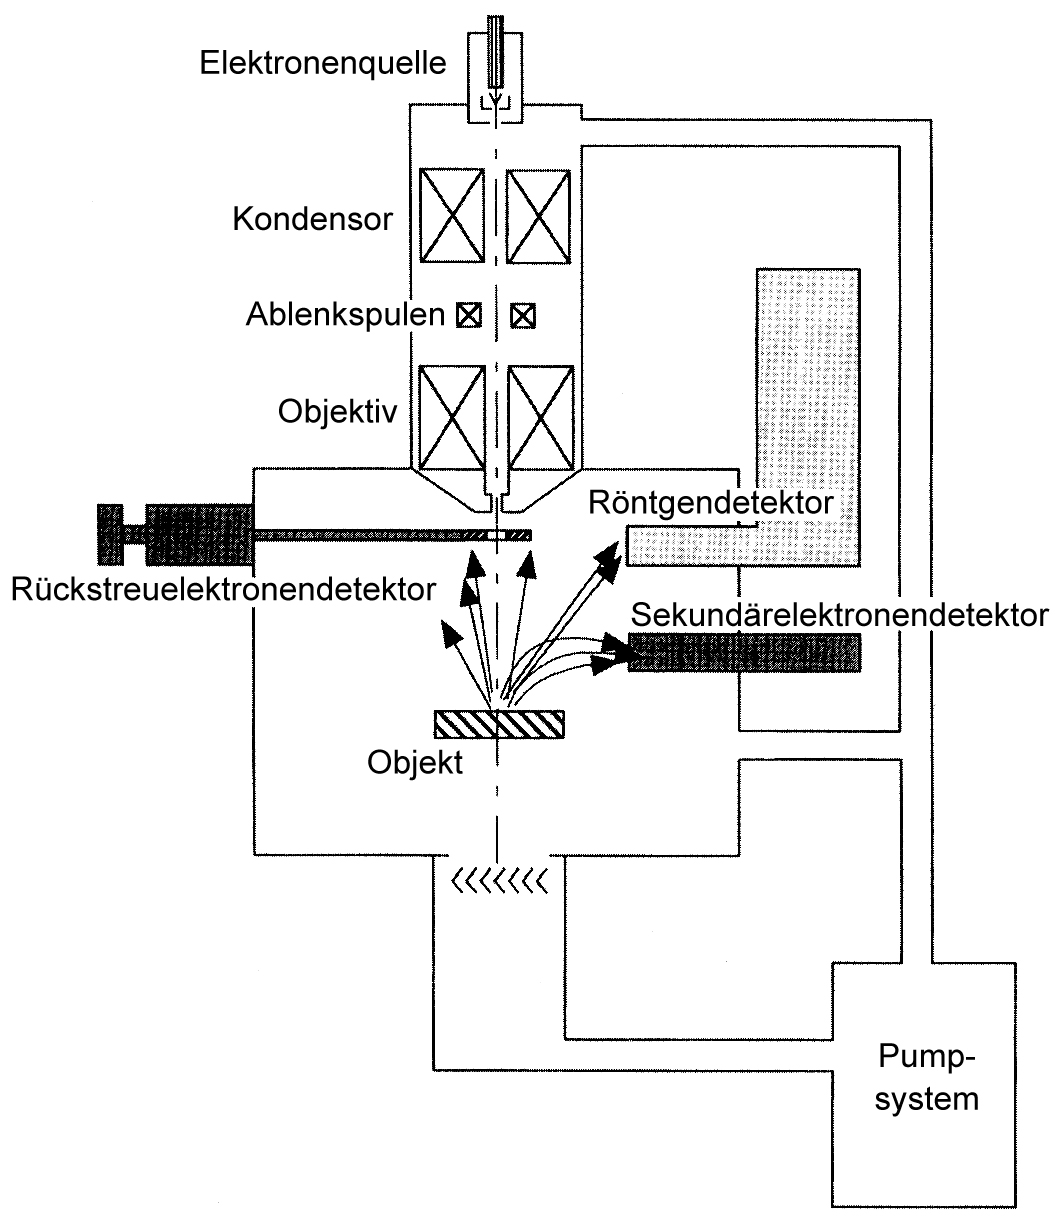
\includegraphics[width=.5\columnwidth]{Grafiken/rem-schema-1.jpg}%
% 
%\caption{Schematischer Aufbau eines REMs \cite{Colliex}.}
%\label{fig:aufbau_rem}
%\end{figure} 


%\subsection{Tiefensch�rfe}
%\label{ch:Grundlagen:sec:REM:sub:Tiefenschaerfe}
%Ein Vorteil des REMs gegen�ber des Lichtmikroskops ist die im Vergleich wesentlich h�here Tiefensch�rfe. Abbildung \ref{fig:schraube} Veranschaulicht diesen Unterschied. 


\begin{figure}%
\centering
%\begin{adjustwidth}{0cm}{0cm}
	\subfloat[Lichtmikroskop]{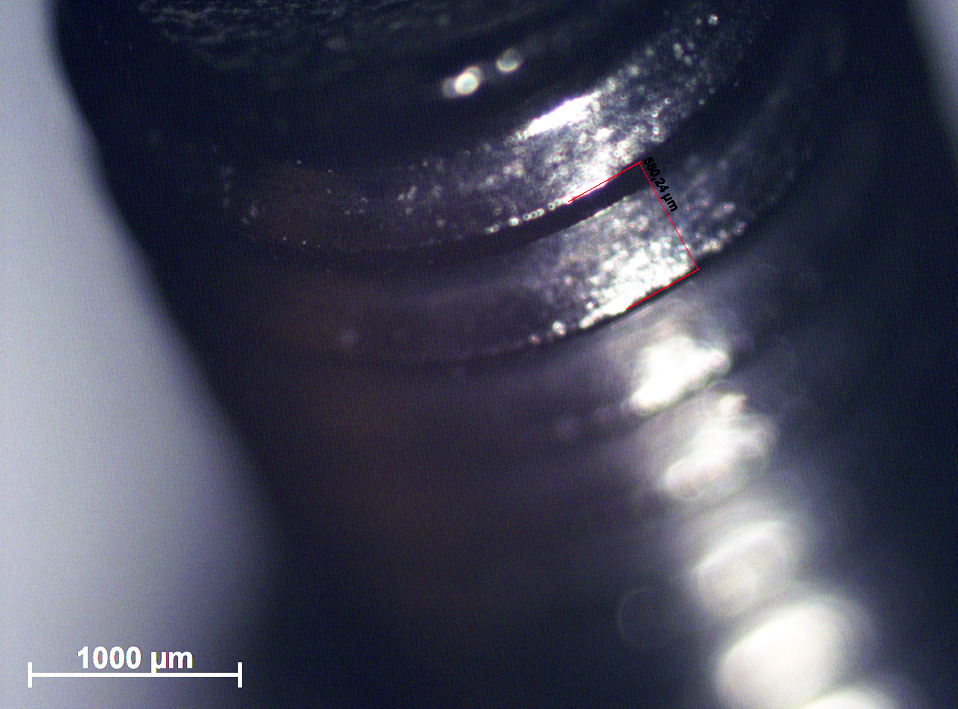
\includegraphics[totalheight=5 cm]{Grafiken/lichtmikroskop_schraube.jpg}\label{fig:schraube_licht}\qquad}
	\subfloat[REM]{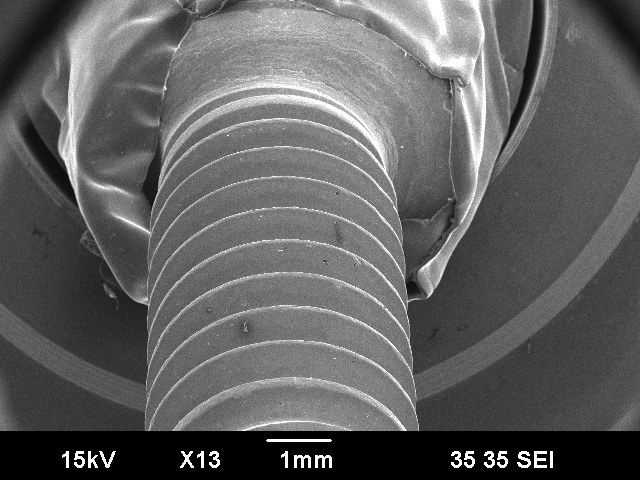
\includegraphics[totalheight=5 cm]{Grafiken/sem_schraube.jpg} \label{fig:schraube_rem}}%
%	\end{adjustwidth}
\caption{Fotos einer Schraube. \textbf{(a)} Unter dem Lichtmikroskop ist eine sehr geringe Tiefensch�rfe zu beobachten. \textbf{(b)} Unter dem REM ist eine hohe Tiefenschr�fe zu beobachten.}%
\label{fig:schraube}%
\end{figure}

%\section{Auswirkungen von REM-Einstellungen}
%
%Das verwendete REM bietet verschiedene Einstellungen, die direkt in der Bedienungsoberfl�che der Kontrollsoftware eingestellt werden k�nnen. F�r das Arbeiten mit dem REM muss eine m�glichst gute Kombination dieser Einstellung f�r das gew�nschte Ergebnis gew�hlt werden.
%
%Abbildung \ref{fig:sem_kv} zeigt SEM Aufnahmen vom Auge einer Fliege bei unterschiedlichen Beschleunigungsspannungen.
%
%
%
%
%\begin{figure}%
%\centering
%%\begin{adjustwidth}{-.5cm}{0cm}
%	\subfloat[5~kV]{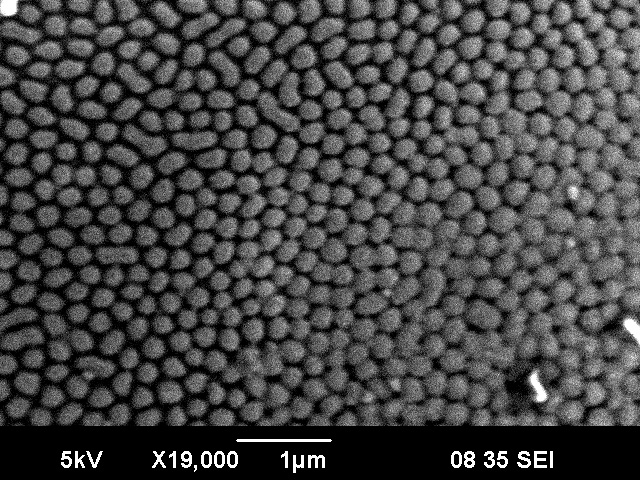
\includegraphics[totalheight=4 cm]{Grafiken/sem_5kv.jpg}\label{fig:sem_5kv}~}
%	\subfloat[15~kV]{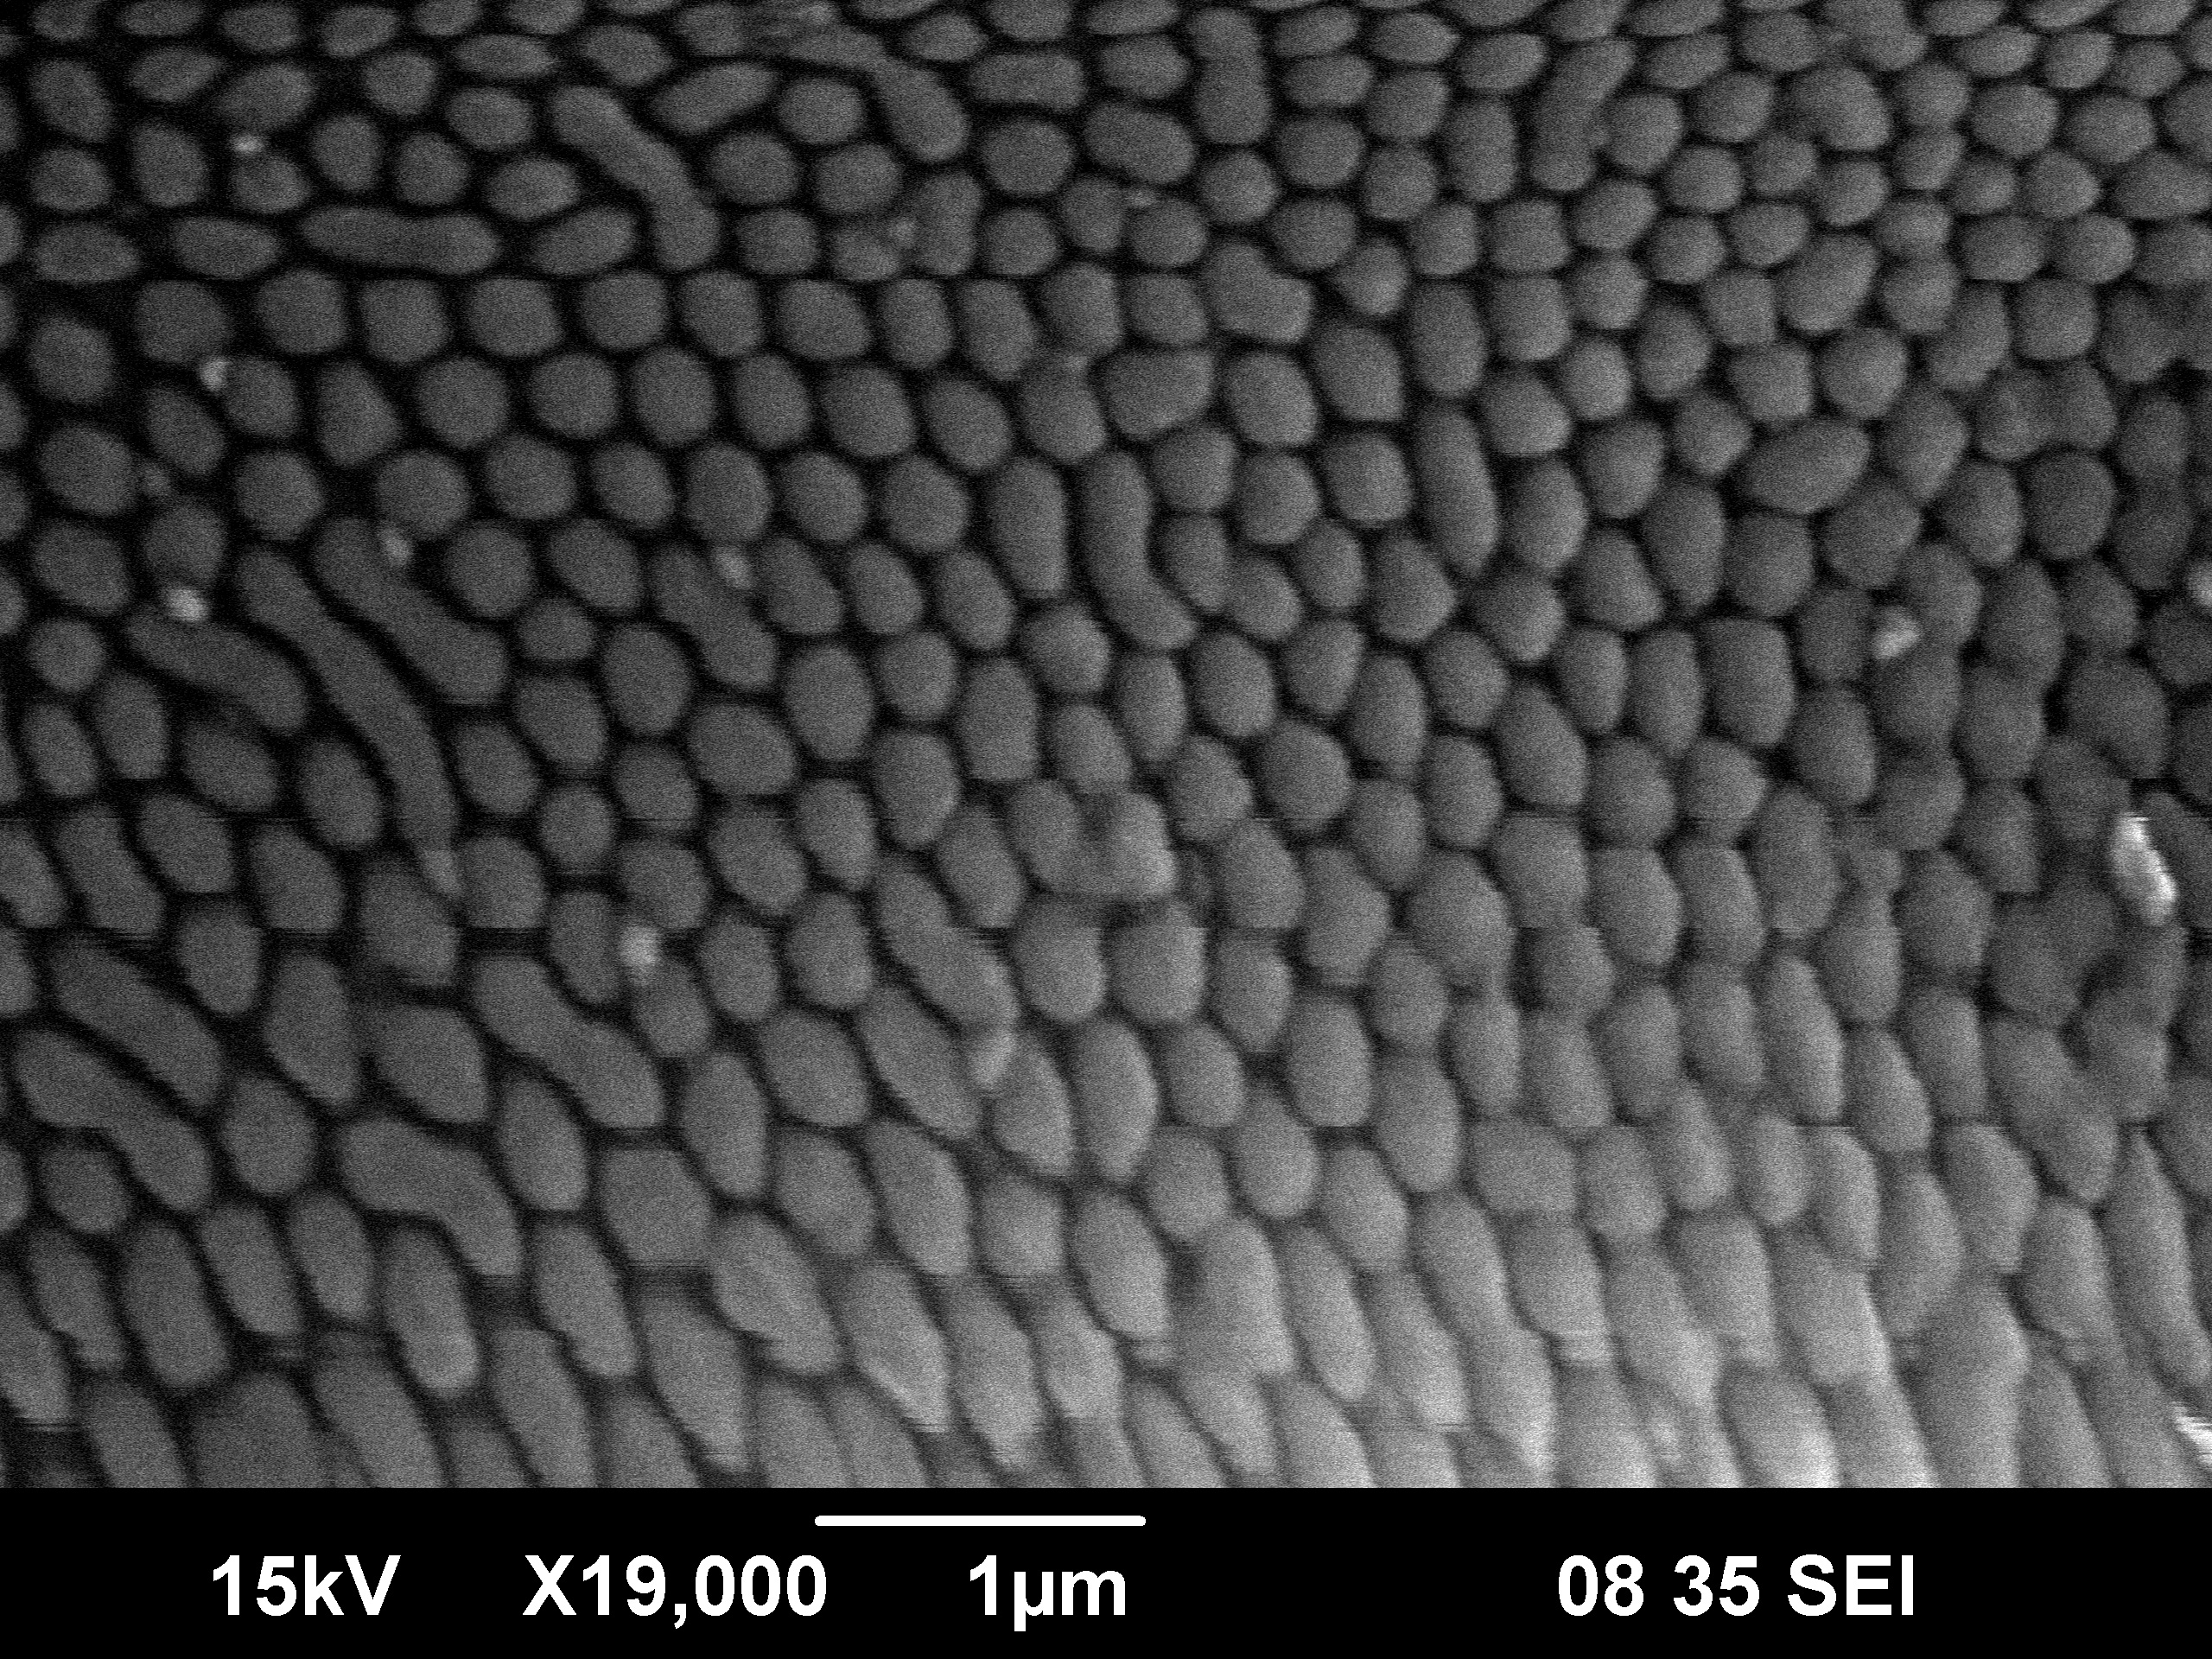
\includegraphics[totalheight=4 cm]{Grafiken/sem_15kv.jpg} \label{fig:sem_15kv}}
%		\subfloat[20~kV]{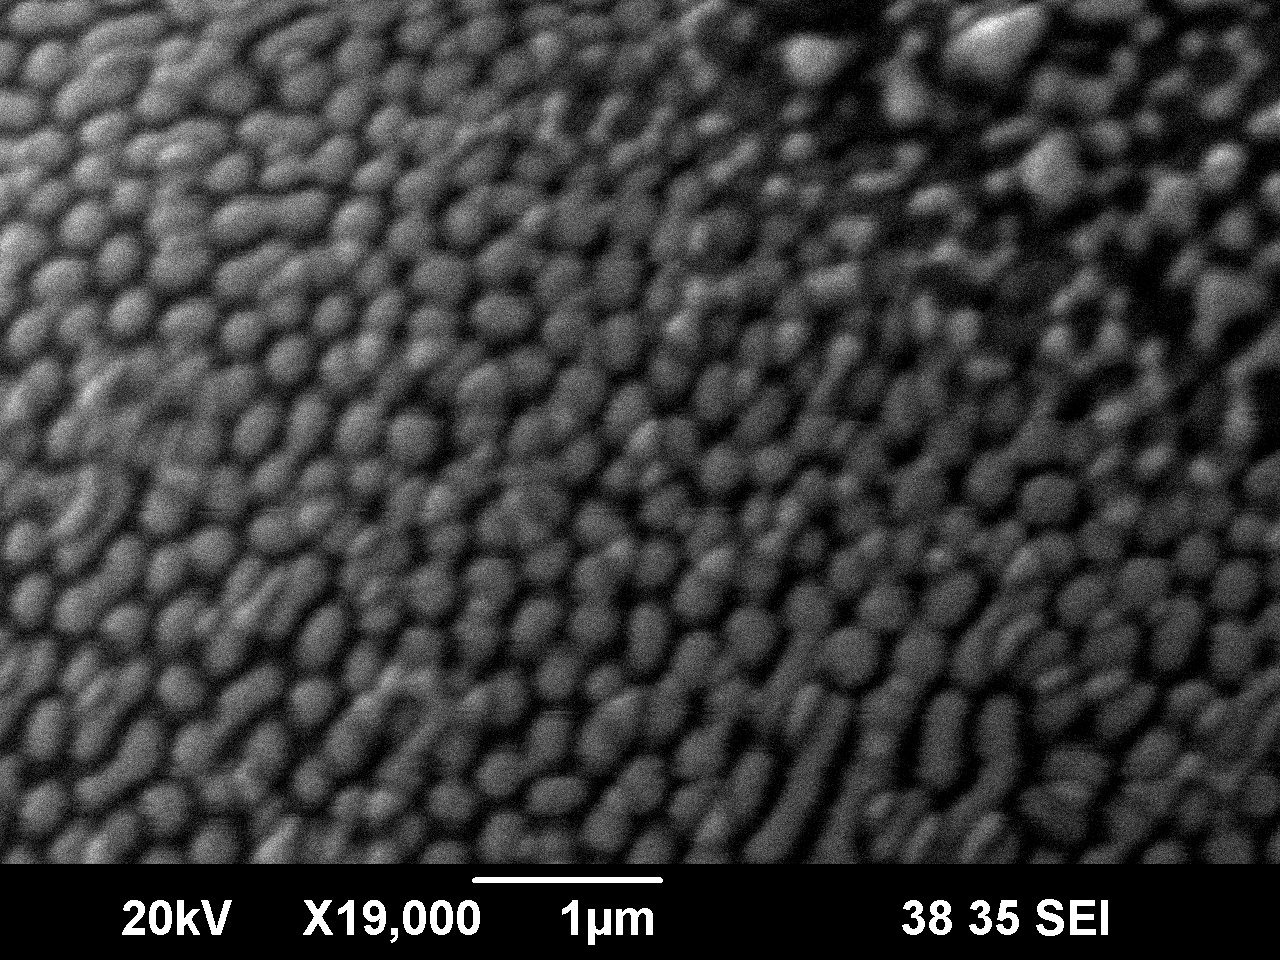
\includegraphics[totalheight=4 cm]{Grafiken/sem_20kv.jpg}\label{fig:sem_20kv}}
%%\end{adjustwidth}
%\caption{Fluoreszenzantworten auf die Laserbestrahlung \cite{Carsten}. \textbf{(a)} An der Glas-Lack-Grenze ist das Ausbilden einer Fluoreszenzantwort zu erkennen. \textbf{(b)} Im Lack ist eine ausgepr�gte Fluoreszenzantwort zu beobachten. \textbf{(c)} An der Lack-Luft-Grenze sind ausgepr�gte Nebenmaxima der Fluoreszenzantwort zu beobachten.}%
%\label{fig:sem_kv}%
%\end{figure}
%

\newpage
\section{Direct Laser Writing}
\label{ch:DLW}
Im Laborversuch wurden Strukturen mit \textit{Direct Laser Writing} (DLW) geschrieben. Dieses Verfahren soll im Folgenden kurz erl�utert werden.

\section{Aufbau und Funktionsweise}
\label{ch:DLW:sec:Aufbau}
Beim DLW erfolgt die Belichtung von fotoempfindlichen Lack �ber einen Laser. Dieser kann �ber ein optisches System in den Fotolack fokussiert werden (vgl. Abbildung \ref{fig:dlw_aufbau}). Der verwendete Fotolack weist eine Empfindlichkeit gegen�ber UV-Strahlung ($\sim$~400~nm) auf. F�r die eingestellte Wellenl�nge des Lasers von 800~nm ist der Fotolack transparent. 

Die Bestrahlung erfolgt durch einen Femtosekundenlaser, der durch ein Mikroskop in den Fotolack fokussiert wird. Femtosekundenlaser werden genutzt, da sie sehr hohe Intensit�ten liefern k�nnen \cite{Nanophotonics}.  Die Probe kann �ber einen Probentisch in $x-$ $y-$ und $z-$ Richtung positioniert werden. Bevor der Strahl in das Mikroskop gef�hrt wird, wird der Strahl aufgeweitet. �ber einen Neutraldichtefilter (ND-Filter) kann die Intensit�t des Lasers gesteuert werden. Ein \textit{Shutter} erm�glicht ein Blockieren des Strahls. Die Steuerung des Systems erfolgt �ber einen PC. Abbildung \ref{fig:dlw_aufbau} veranschaulicht den Aufbau schematisch.


\begin{figure}%
\centering
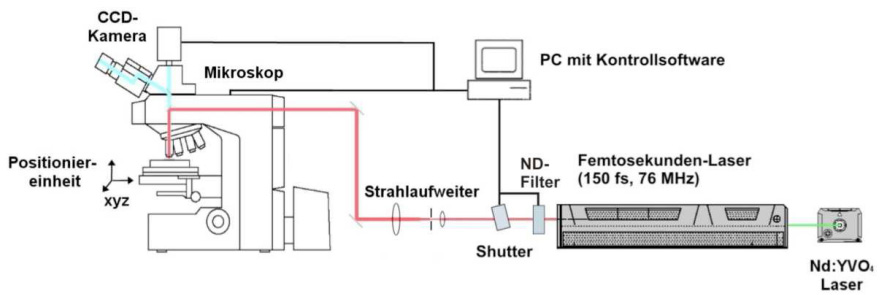
\includegraphics[width=.9\columnwidth]{Grafiken/dlw_aufbau.jpg}%
\caption{Schematischer Aufbau eines DLW-Systems \cite{Versuchsanleitung}.}%
\label{fig:dlw_aufbau}%
\end{figure}

Im Fokuspunkt findet eine eine zwei-Photonen-Absorption (engl. \textit{two-photon absorption} - TPA)  statt, die zu einer zwei-Photonen-Polymerisation (2PP) f�hrt.
Abbildung \ref{fig:2PP} zeigt schematisch den Unterschied zwischen ein-Photonen-Absorption und zwei-Photonen-Absorption.
So kann ein Atom durch ein Photon angeregt werden, wenn die Energie des Photons $E~=h\nu$ ausreicht um die Energiedifferenz zwischen den beiden Energieniveaus S$_1$ und S$_0$ zu �berwinden. In der Abbildung ist Strahlung im UV-Bereich notwendig ($\lambda \approx 400$~nm). Bei einer Laserwellenl�nge von 800~nm reicht die Energie eines Photons nicht aus um das Atom anzuregen.
Mit TPA ist dies m�glich. Hierbei k�nnen zwei Photonen gleichzeitig absorbiert werden, deren addierte Energien $E_{\mbox{ges}}=2h\nu$ ausreichen um die Energiedifferenz zwischen den Energieniveaus S$_2$ und S$_0$ zu �berwinden.

\begin{figure}[h]%
\centering
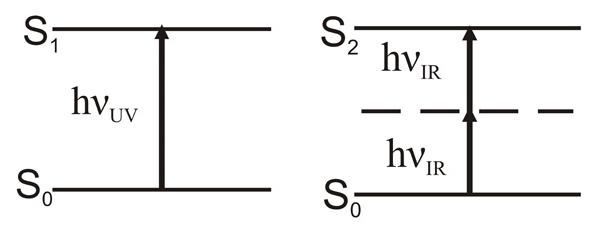
\includegraphics[width=.4\columnwidth]{Grafiken/2PP.JPG}%
\caption{Vergleich ein- und zwei-Photonen-Absorption \cite{Nanophotonics}.}%
\label{fig:2PP}%
\end{figure}
\enlargethispage{\baselineskip}
Da die Wahrscheinlichkeit von TPA quadratisch von der Laserintensit�t abh�ngt finden die TPA Prozesse im Fokus des Lasers statt \cite{Nanophotonics}. 
Durch TPA wird eine fotoaktive Komponente im Lack aktiviert, was zur Entstehung einer S�ure f�hrt, die beim sp�teren \textit{Post Exposure Bake} (PEB) als Katalysator f�r die Polymerisation dient \cite{Carsten}.  \todo{Den vorherigen Satz nchmal lesen ob das passt mit dem was Carsten geschrieben hat.} Somit kann ein beliebiger Punkt im Lackvolumen fokussiert werden und dreidimensionale Strukturen geschrieben werden. Ein geschriebener Volumenpixel wird Voxel genannt. 

Um die Polymerisation beim 2PP-Prozess zu starten, muss eine gewisse Polymerisationsschwelle �berwunden werden. Erst wenn die Laserintensit�t diese Schwelle �berschreitet, kommt es zur Polymeisation. 
Dadurch ist es m�glich Strukturen unterhalb der Aufl�sungsgrenze (vgl. \eqref{eq:Abbe}) herzustellen. Abbildung \ref{fig:poly} veranschaulicht dies. F�r gro�e Intensit�ten folgt ein gro�er Voxeldurchmesser. F�r Intensit�ten  nahe der Polymerisationsschwelle folgen sehr kleine Voxeldurchmesser. F�r Intensit�ten unterhalb der Polymerisationsschwelle erfolgt keine Polymerisation.
\enlargethispage{\baselineskip}
\begin{figure}%
\centering
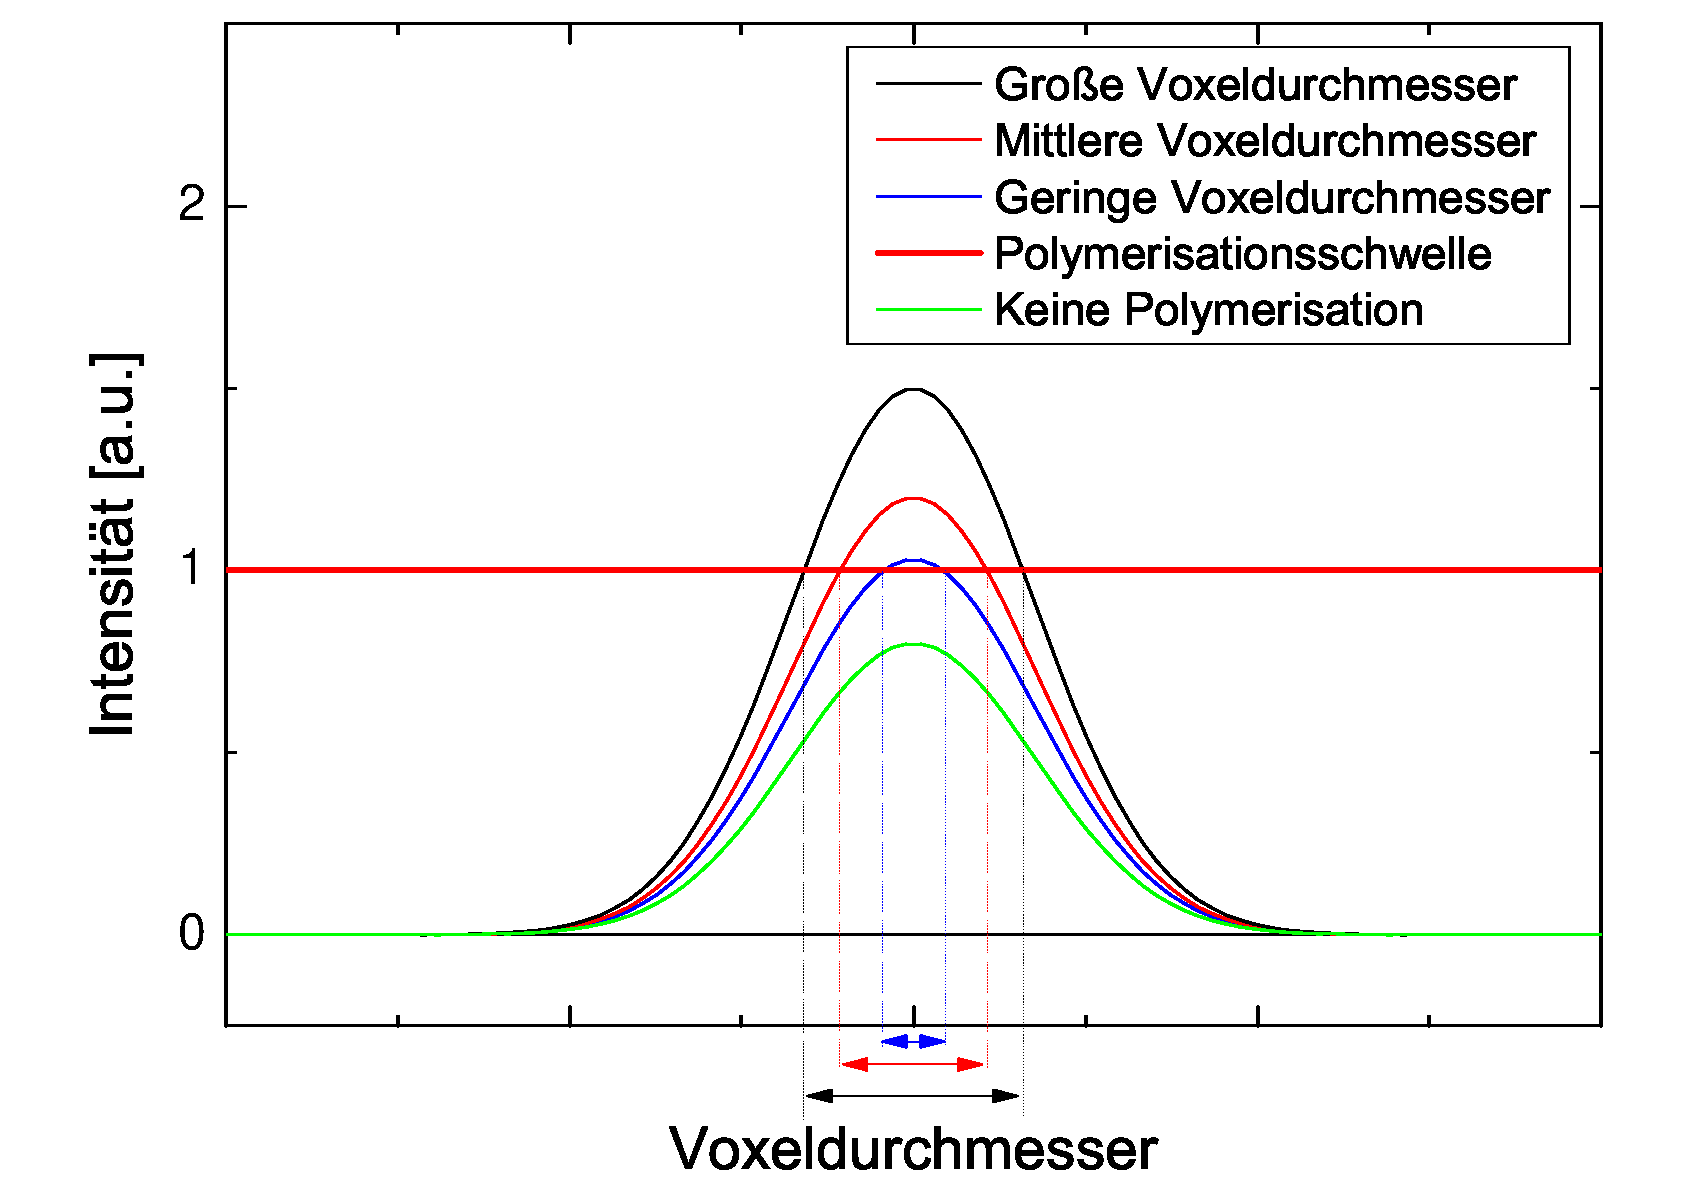
\includegraphics[width=.5\columnwidth]{Grafiken/Polymer.pdf}%
\caption{Schematische Darstellung der Abh�ngigkeit des Voxeldurchmessers von der Intensit�t \cite{Nanophotonics}.}%
\label{fig:poly}%
\end{figure}

\begin{figure}%
\centering
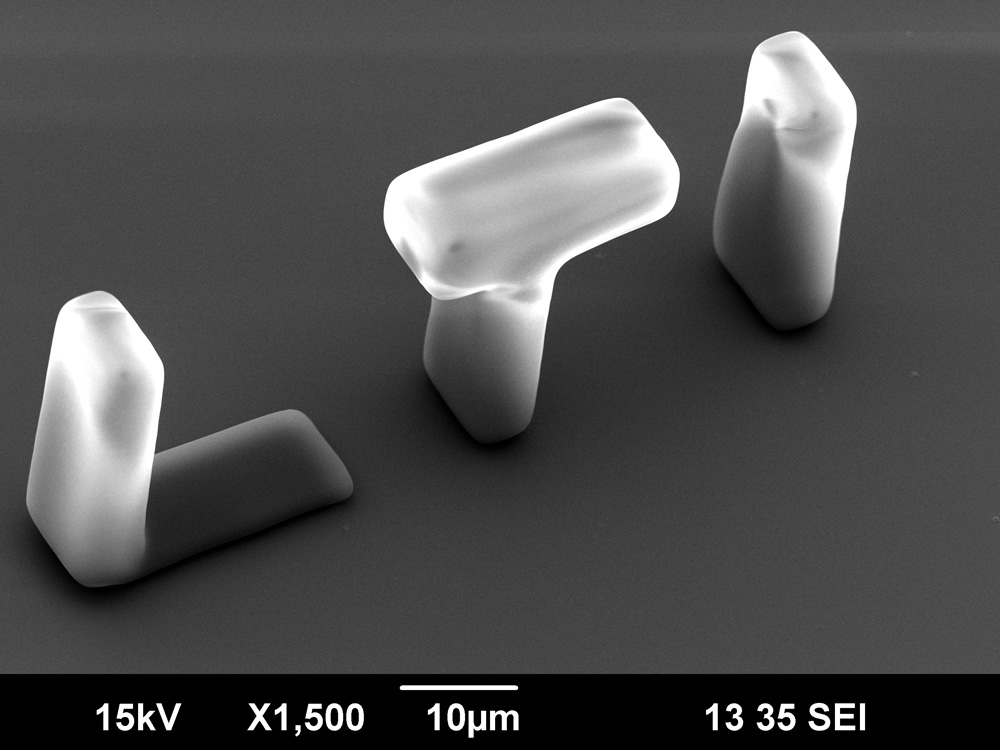
\includegraphics[width=.39\columnwidth]{Grafiken/LTI.jpg}%
\caption{REM Aufnahme dreidimensionaler Strukturen die mit DLW geschrieben wurden.}%
\label{fig:LTI}%
\end{figure}

Abbildung \ref{fig:LTI} veranschaulicht die M�glichkeit dreidimensionale Strukturen mit DLW zu schreiben. 


%% ===========================
\chapter{Probenherstellung}
\label{ch:Herstellun}

Zur Herstellung der Proben wurde auf ein gereinigtes Glassubstrat mit einem \textit{Spin Coater} ein Fotolackfilm (SU-8) aufebracht. Um das L�sungsmittel aus dem Lack zu treiben, wurde die Probe f�r 9 Minuten bei 95~�C auf einer \textit{Hot Plate} gebacken (\textit{Soft Bake}) \cite{Versuchsanleitung, Carsten}. Anschlie�end wurden der Lack an den R�ndern der Probe entfernt. Diese Probenvorbereitung erfolgte durch den Versuchsbetreuer.

Bevor die Strukturen mit DLW in den Fotolack geschrieben wurden, erfolgte die Kalibrierung der Laserintensit�t des DLW-Systems mit Hilfe einer Fotodiode. Dazu wurde die Laserleistung auf $\sim$3,4~mW eingestellt und die automatisierte Kalibrierung gestartet.
%\todo{Vorherigen Satz einmal Lesen und gucken ob passt.}

Zur Belichtung des Lacks wurde die Probe in das DLW-System eingebaut. Das Objektiv des zur Belichtung verwendeten Mikroskops wurde mit Immersions�l in Kontakt zum Glassubstrat gebracht. 

Um Verkippungen der Probe auszugleichen wurde an drei Punkten die Glas-Lack-Grenze bestimmt. Dazu wurde der Laserfokus manuell in $z$-Richtung durch die Probe bewegt und dabei das Fluoreszenzsignal beobachtet. 

\begin{figure}%
\centering
%\begin{adjustwidth}{-.5cm}{0cm}
	\subfloat[Glas-Lack]{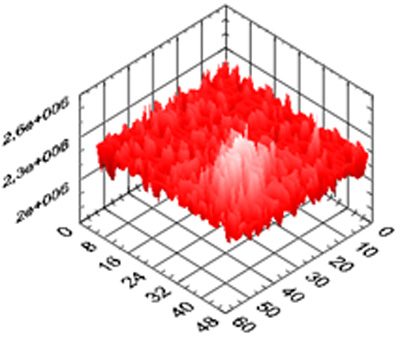
\includegraphics[totalheight=4 cm]{Grafiken/glass_su8.jpg}\label{fig:glas_lack}}
	\subfloat[Lack]{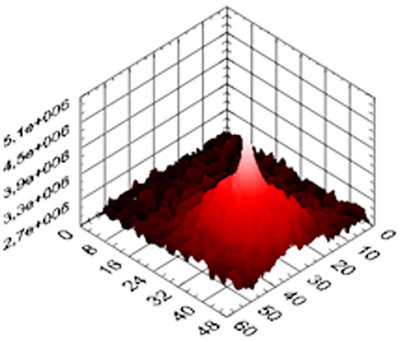
\includegraphics[totalheight=4 cm]{Grafiken/su8.jpg} \label{fig:lack}}%
		\subfloat[Lack-Luft]{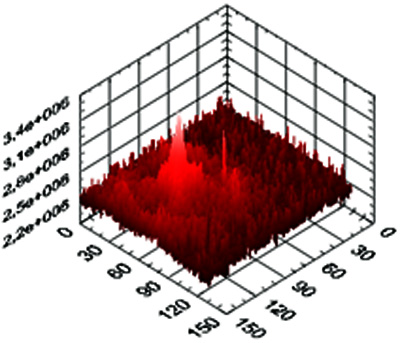
\includegraphics[totalheight=4 cm]{Grafiken/su8_luft.jpg}\label{fig:lack_luft}}
%\end{adjustwidth}
\caption{Fluoreszenzantworten auf die Laserbestrahlung \cite{Carsten}. \textbf{(a)} An der Glas-Lack-Grenze ist das Ausbilden einer Fluoreszenzantwort zu erkennen. \textbf{(b)} Im Lack ist eine ausgepr�gte Fluoreszenzantwort zu beobachten. \textbf{(c)} An der Lack-Luft-Grenze sind ausgepr�gte Nebenmaxima der Fluoreszenzantwort zu beobachten.}%
\label{fig:fluoreszenz}%
\end{figure}

Abbildung \ref{fig:fluoreszenz} zeigt die Fluoreszenzantworten bei einer Fokussierung des Lasers auf die Glas-Lack-Grenze (Abbildung \ref{fig:glas_lack}), in die Lackschicht (Abbildung \ref{fig:lack}) sowie auf die Lack-Luft-Grenze (Abbildung \ref{fig:lack_luft}). An der Glas-Lack-Grenze ist die Ausbildung einer Fluoreszenzantwort zu erkennen. Befindet sich der Laserfokus im Lack ist eine ausgepr�gte Fluoreszenzantwort zu beobachten. An der Lack-Luft-Grenze ist das Ausbilden von Nebenmaxima zu erkennen. 
Anhand dieses Verfahrens wurden die Glas-Lack-Grenze bestimmt und eingestellt.

Anschlie�end wurden die vom Versuchsbetreuer vorbereiteten Strukturen in den Lack geschrieben. Abbildung \ref{fig:Strukturen} zeigt die geschriebenen Strukturen. Hier sind Linien einzelner Voxel (links), ein dreidimensionales LTI-Logo (mitte) sowie Gitterstrukturen (rechts) zu erkennen. Der Schreibdauer der Strukturen betr�gt etwa 2 Stunden.

\begin{figure}%
\centering
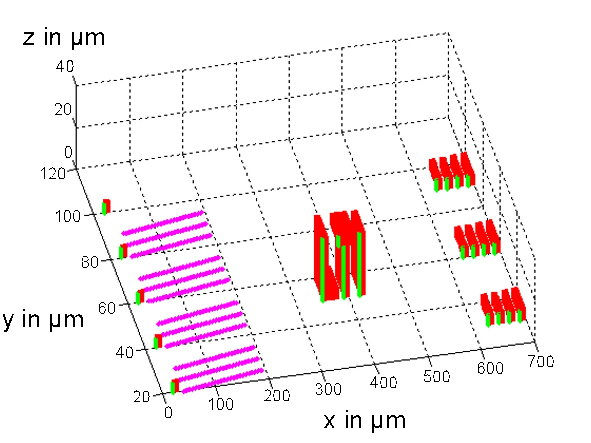
\includegraphics[width=.5\columnwidth]{Grafiken/Strukturen.pdf}%
\caption{Vorlage der geschriebenen Strukturen \cite{Carsten}.}%
\label{fig:Strukturen}%
\end{figure}


Nach der Belichtun des Fotolacks erfolgte ein $Post~Exposure~Bake$ (PEB) f�r 7~Minuten bei 95~�C auf einer $Hot~Plate$. Bei diesem Backvorgang werden zuvor belichtete Bereiche des Lacks quervernetzt und damit unempfindlich gegen�ber dem Entwickler. Anschlie�end erfolgte die Entwicklung mit dem Entwickler \mbox{mr-Dev 600}. 
Die Probe wurde f�r 7~Minuten im Entwickler geschwenkt, zum stoppen der Entwicklung mit Isopropanol abgesp�hlt und mit Stickstoff getrocknet. Nach einer optischen Kontrolle der Probe wurde die Probe f�r eine weitere Minute in \mbox{mr-Dev 600} nachentwickelt. Bei der Entwicklung werden die zuvor nicht belichteten Lackbereiche entfernt.

Um die Lackstrukturen weiter zu festigen wurde die Probe f�r 10 Minuten bei 150~�C auf einer $Hot~Plate$ gebacken ($Hard~Bake$). Bei diesem $Hard~Bake$ werden au�erdem Isopropanolreste aus den Strukturen ausgetrieben. Dies ist notwendig, damit es beim sp�ter durchgef�hrten Aufsputtern von Gold zu keiner Zerst�rung der Strukturen durch das Plasma kommt.

Die Abscheidung von Gold erfolgte in einer Hochfrequenz (engl. $radio~frequency$ - RF)-Sputteranlage. Die Goldschicht dient dazu Aufladungseffekte auf den nicht leitf�higen Lackstrukuturen w�hrend dem Betrachten unter dem REM zu verhindern.
 

\chapter{Auswertung der Messergebnisse}
\label{ch:Auswertung}

Die Charakterisierung der hergestellten Strukturen erfolgte mit Hilfe eines REMs. Im Folgenden wird die Voxelgr��e in Abh�ngigkeit von Belichtungszeit und Laserleistung untersucht. Die Polymerisationsschwelle wird bestimmt und der Einfluss benachbarter Linien aufeinander untersucht.

\section{Bestimmung der Voxelgr��e}
\label{ch:Auswertung:sec:voxel}

Um die Voxelausdehnung in $z$-Richtung zu bestimmen, wurden einzelne Voxel nebeneinander geschrieben. Hierbei wurde die Position in $z$-Richtung mit jedem Voxel um 100~nm erh�ht. Abbildung \ref{fig:steigung} zeigt dies Schematisch. Der Laser ist zuerst in das Glassubstrat fokusiert. Der Fokus verschiebt sich mit jedem Voxel nach oben. Sobald sich der Fokus im Fotolack befindet, wird dieser belichtet. Nach dem Entwickeln verbleiben nur die Voxel stehen, die direkten Kontakt zum Glassubstrat haben. In Abbildung \ref{fig:steigung} w�rde somit der erste Laserfokuspunkt kein Voxel bilden, das Voxel des letzten Fokuspunktes w�rde beim Entwickeln wegschwimmen. Aus der Anzahl der verbleibenden Voxel l�sst sich damit Voxelausdehnung in $z$-Richtung absch�tzen.

\begin{figure}%
\centering
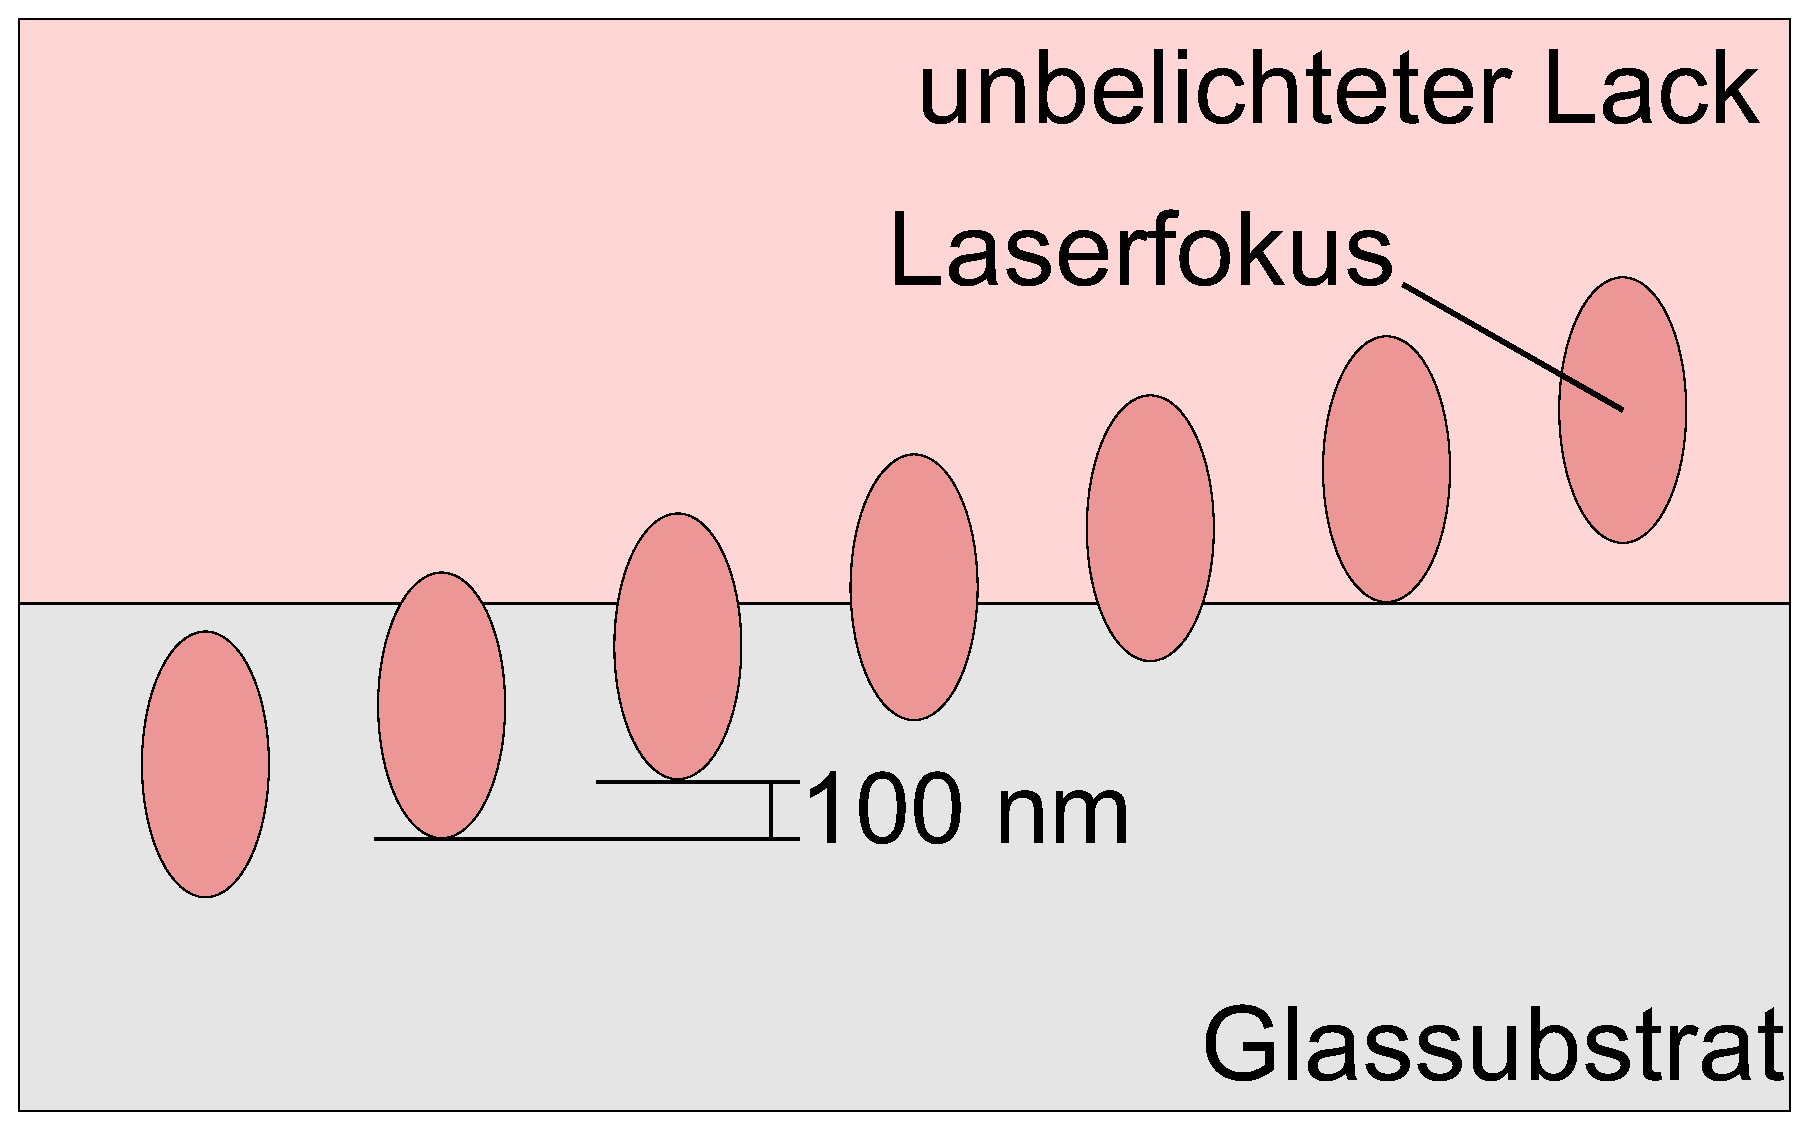
\includegraphics[width=.4\columnwidth]{Grafiken/Steigung.pdf}%
\caption{Schematische Darstellung: Bestimmung der Voxelausdehnung in $z$-Richtung.}%
\label{fig:steigung}
\end{figure}
\enlargethispage{\baselineskip}
Abbildung \ref{fig:voxelausdehnung} zeigt eine REM-Aufnahme der geschriebenen Voxelstrukturen. Es wurde eine Laserleistung von 1,75~mW verwendet. Die Belichtungszeit pro Voxelzeile betr�gt (Zeilenweise, von unten nach oben) 10~ms, 20~ms und 30~ms. In der untersten Reihe sind 8 Voxel zu erkennen. Daraus l�sst sich eine Voxelausdehnung in $z$-Richtung von $\sim$800~nm absch�tzen. In Tabelle \ref{tab:Voxel} sind die Voxelgr��en in Abh�ngigkeit der Energie zu finden.

Um die Voxelausdehnung in $x$- bzw. $y$-Richtung zu bestimmen, wurde das jeweils letzte Voxel einer Reihe vermessen. Bei diesen Voxeln ist bei einer Aufsicht die volle Voxelbreite zu messen. Abbildung \ref{fig:voxel_x} zeigt die Aufsicht auf ein Voxel (Laserleistung: 1,75~W, Belichtungszeit: 30~ms). Zu erkennen ist eine elliptische Form. Zu erwarten w�re eine kreisf�rmige Form \cite{Multiphoton}. Dies ist vermutlich auf eine astigmatische Aberration des Linsensystems beim Schreiben der Strukturen zur�ckzuf�hren. 
Zur Bestimmung der Voxelbreite wurde die k�rzere Achse der Ellipse gew�hlt. F�r das in der Abbildung gezeigte Voxel ergibt sich damit eine laterale Breite von $\sim$1,14~$\upmu$m. Tabelle \ref{tab:Voxel} beinhaltet auch die laterale Breite der Voxel in Abh�ngigkeit der Energie.
Abbildung \ref{fig:voxel} veranschaulicht den Zusammenhang zwischen Energie und der Voxelbreite. Mit steigender Energie steigt auch die Voxelbreite. Dies best�tigt das in Kapitel \ref{ch:DLW} beschriebene Verhalten der minimalen Aufl�sung.
%Es zeigt sich weitergehend, dass die Belichtungszeit nicht linear in die Voxelbreite eingeht.


%\begin{figure}%
%\centering
%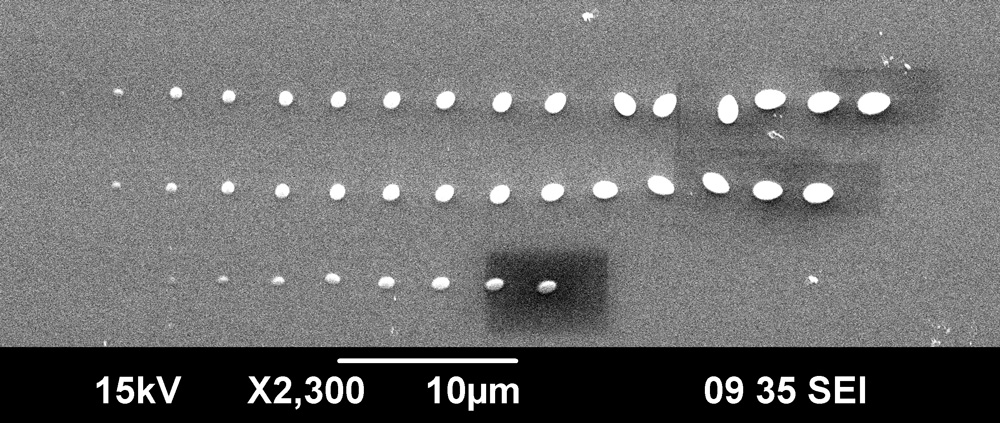
\includegraphics[width=.8\columnwidth]{Grafiken/voxel_bsp.jpg}%
%\caption{REM Aufnahme der Voxelstrukturen.}%
%\label{fig:voxelausdehnung}%
%\end{figure}
%



\begin{figure}%
\centering
%\begin{adjustwidth}{-.5cm}{0cm}
	\subfloat[Voxelanordnung]{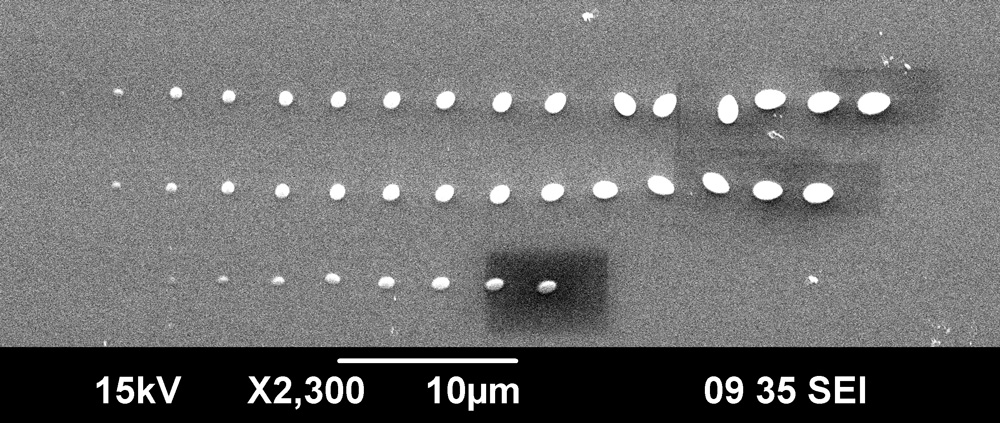
\includegraphics[totalheight=4 cm]{Grafiken/voxel_bsp.jpg}\label{fig:voxelausdehnung}\qquad}
	\subfloat[Voxelgr��e]{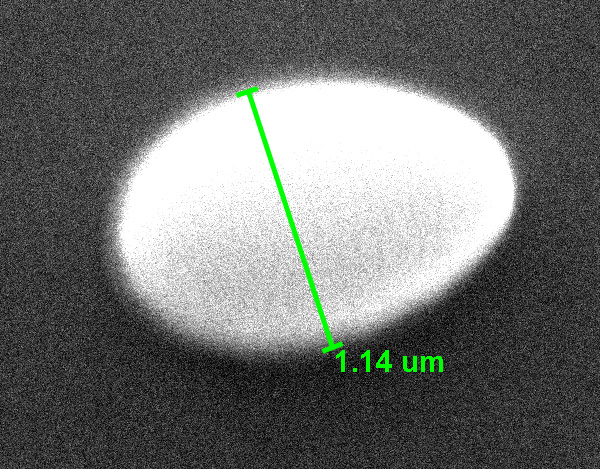
\includegraphics[totalheight=4 cm]{Grafiken/voxel_x.jpg} \label{fig:voxel_x}}%
%\end{adjustwidth}
\caption{REM Aufnahmen der Voxelstrukturen}%
\label{fig:voxel_subfig}%
\end{figure}

\begin{figure}%
\centering
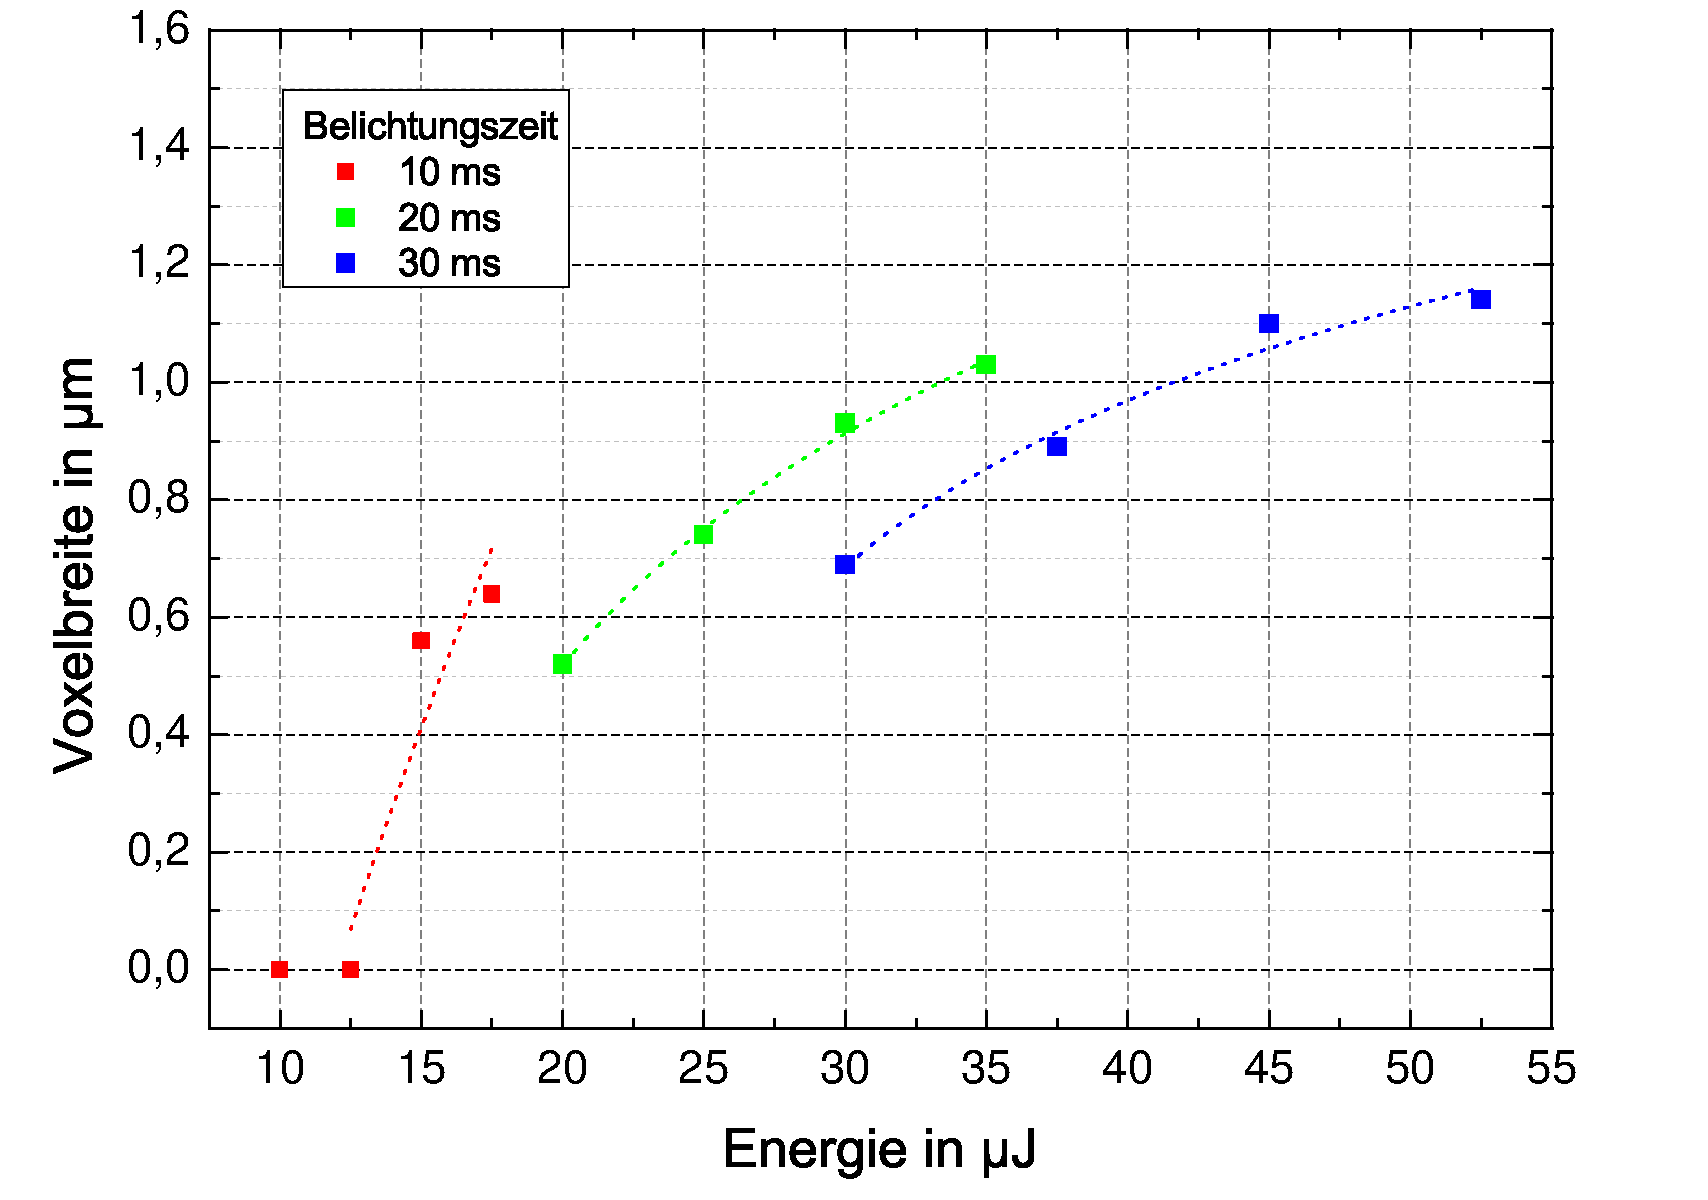
\includegraphics[width=.7\columnwidth]{Grafiken/Voxel.pdf}%
\caption{Voxelbreite in Abh�ngigkeit der Energie. Zur Veranschaulichung der mit der Energie steigenden Voxelgr��e wurden Orientierungslinien eingezeichnet.}%
\label{fig:voxel}%
\end{figure}
%\begin{figure}%
%\centering
%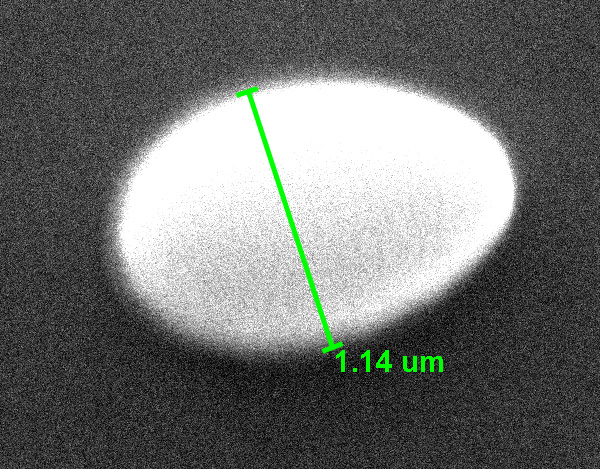
\includegraphics[width=\columnwidth]{Grafiken/voxel_x.jpg}%
%\caption{}%
%\label{}%
%\end{figure}

\section{Bestimmung der Polymerisationsschwelle}
\label{ch:Auswertung:sec:Polymerisation}

Zur Bestimmung der Polymerisationsschwelle wurden einzelne Voxel mit verschiedenen Belichtungszeiten und Laserleistungen geschrieben (vgl. Abbildung \ref{fig:voxelausdehnung}). Es wurden Leistungen von 1~mW bis 1,75~mW, Belichtungszeiten von 10~ms bis 30~ms und daraus resultierend Energien von 10~$\upmu$J bis $\sim$50~$\upmu$J untersucht (vgl. Tabelle \ref{tab:Voxel}). Aus der Tabelle sowie Abbildung \ref{fig:voxel} geht hervor, dass bis zu einer Energie von 12,5~$\upmu$J keine Voxel geschrieben werden. Ab 15~$\upmu$J sind Voxel zu erkennen. Die Polymerisationsschwelle befindet sich also bei einer Energie zwischen $12,5~\upmu$J$~<E_{\mathrm{Schwelle}}<15~\upmu$J.

Zudem ist zu erkennen, dass bei gleicher Energie mit unterschiedlicher Belichtungszeit eine unterschiedliche Voxelgr��e resultiert. Die Belichtungszeit wirkt also nicht linear auf die Voxelgr��e aus. Dies ist in Abbildung \ref{fig:voxel} zum Beispiel bei 30~$\upmu$J zu erkennen.

\begin{table}%
\centering
% \renewcommand{\arraystretch}{1.3}
\caption{Belichtungsparameter und daraus resultierende Voxelgr��en.}
\begin{tabular}{lllllll}
\toprule
 
Leistung&Zeit&Energie&Anzahl&H"ohe &Breite&Volumen\\
in mW&in ms&in $\upmu$J&Voxel&in $\upmu$m&in $\upmu$m&in $\upmu$m$^3$\\
\midrule
1,75&10&17,5&8&0,80&0,67&0,19\\
1,75&20&35,0&14&1,40&1,03&0,78\\
1,75&30&52,5&15&1,50&1,14&1,02\\
1,50&10&15,0&3&0,30&0,56&0,05\\
1,50&20&30,0&13&1,30&0,93&0,59\\
1,50&30&45,0&15&1,50&1,10&0,95\\
1,25&10&12,5&0&0,00&0,00&0,00\\
1,25&20&25,0&9&0,90&0,74&0,26\\
1,25&30&37,5&11&1,10&0,89&0,46\\
1,00&10&10,0&0&0,00&0,00&0,00\\
1,00&20&20,0&4&0,40&0,52&0,06\\
1,00&30&30,0&9&0,90&0,69&0,22\\

\bottomrule 
\end{tabular}

\label{tab:Voxel}
\end{table}



\section{Gitterstrukturen}
\label{ch:Auswertung:sec:ProblemeGitter}

Beim Betrachten der Gitterstrukturen in Abbildung \ref{fig:Gitter_uebersicht}{ zeigt sich, dass im Gegensatz zur Vorlage (vgl. Abbildung  \ref{fig:Strukturen}) auf der fertigen Probe nicht alle Strukturen vorhanden sind.

Die Strukturen in Abbildung \ref{fig:Gitter_uebersicht} wurden zeilenweise mit unterschiedlicher Laserleistung (von unten nach oben: 1,75~mW, 1,5~mW und 1,25~mW), spaltenweise mit unterschiedlichen Linienabst�nden (von links nach rechts: 1~$\upmu$m, 0,75~$\upmu$m, 0,5~$\upmu$m und 0,25~$\upmu$m) geschrieben. Die Linien wurden mit einer Geschwindigkeit von 1~mm/s im Vektor-Modus geschrieben. 

Bei einer Leistung von 1,75~mW reicht die Energie aus, um die Polymerisationsschwelle des Lackes zu �berwinden. Es sind alle 4 Gitterstrukturen zu erkennen. Das Fehlen einiger Strukturen bei geringeren Leistungen ist darauf zur�ckzuf�hren, dass die Polymerisationsschwelle nicht �berschritten wird. 

Es zeigt sich allerdings, dass bei geringerem Abstand zwischen den Linien Strukturen bei Leistungen vorhanden sind, die bei gr��eren Linienabst�nden nicht vorhanden sind. Durch den geringeren Linienabstand kommt es beim Schreiben einer Linie zur Belichtung von benachbarten Linien. Dadurch kann die Polymerisationsschwelle �berschritten werden. 

Abbildung \ref{fig:Gauss1} zeigt schematisch zwei benachbarte Linien, bei denen die Polymerisationsschwelle nicht �berschritten wird. Werden die beiden Linien n�her zusammengebracht (Abbildung \ref{fig:Gauss2}) kommt es zu einer �berlagerung beider, und die Polymerisationsschwelle kann �berschritten werden.

\begin{figure}%
\centering
%\begin{adjustwidth}{0cm}{0cm}
	\subfloat[Gitterstrukturen]{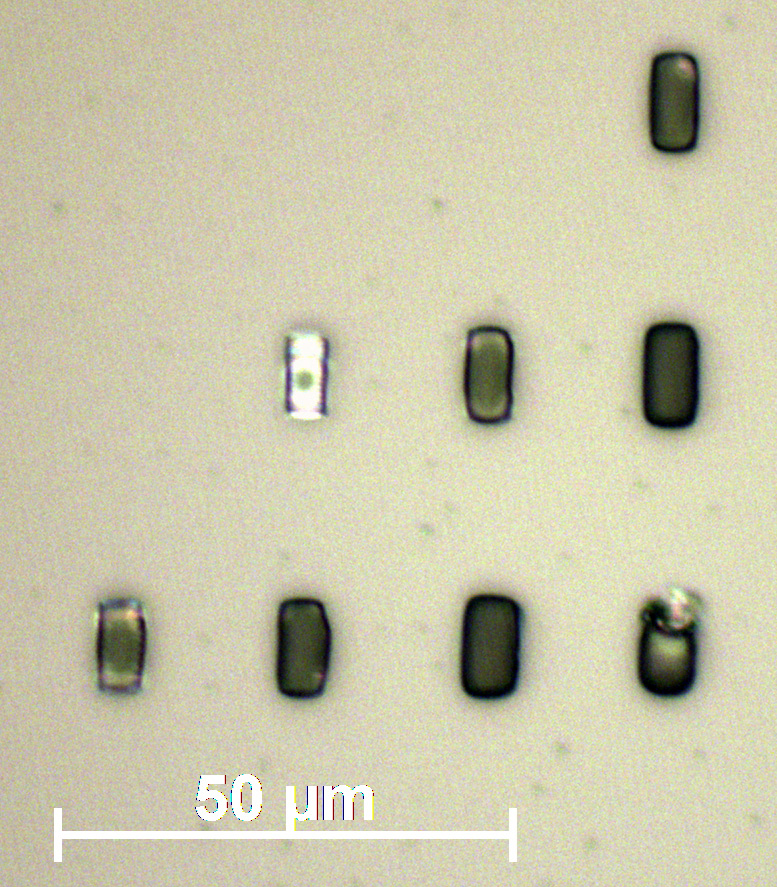
\includegraphics[totalheight=5 cm]{Grafiken/Gitter_uebersicht.jpg}\label{fig:Gitter_uebersicht}\qquad}
	\subfloat[Struktur]{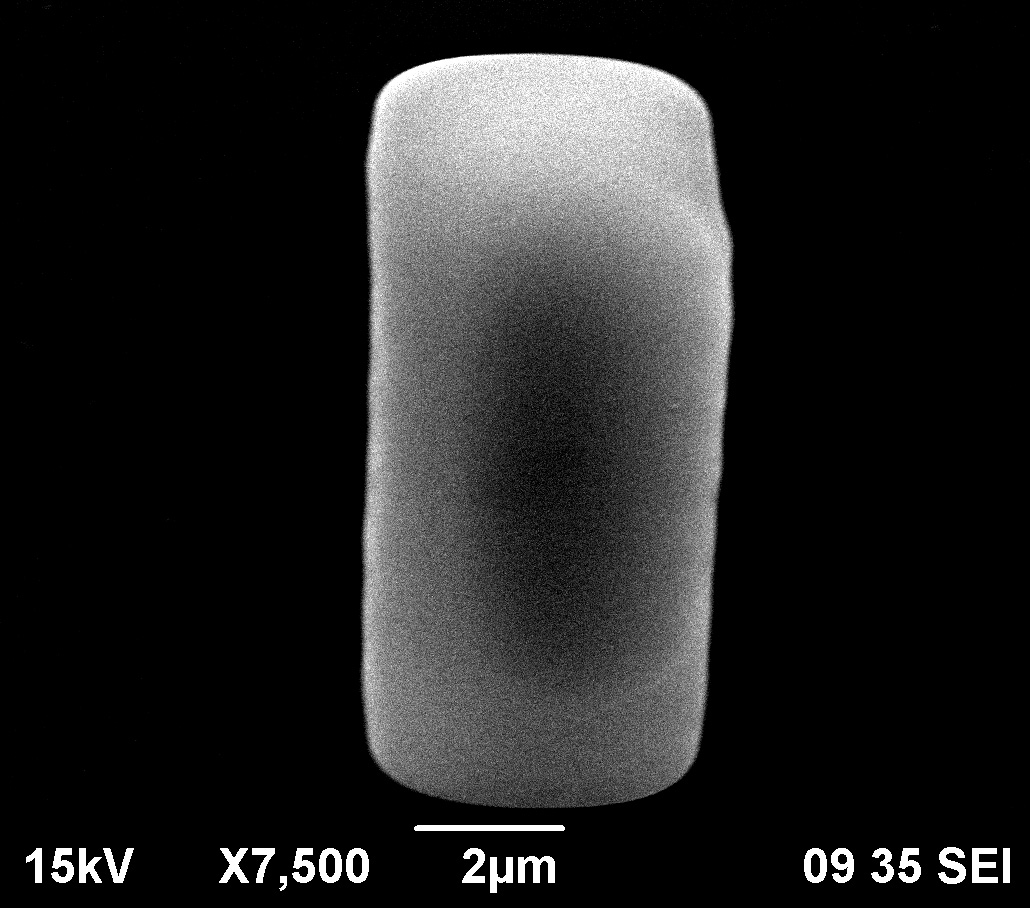
\includegraphics[totalheight=5 cm]{Grafiken/Gitter.jpg} \label{fig:Gitter}}%
%\end{adjustwidth}
\caption{\textbf{(a)} Lichtmikroskopische Aufnahme der geschriebenen Gitterstrukturen. \textbf{(b)} REM-Aufnahme: Die Gitterstruktur konnte nicht aufgel�st werden.}%
\label{fig:voxel_subfig}%
\end{figure}


\begin{figure}%
\centering
\begin{adjustwidth}{-.50cm}{0cm}
	\subfloat[]{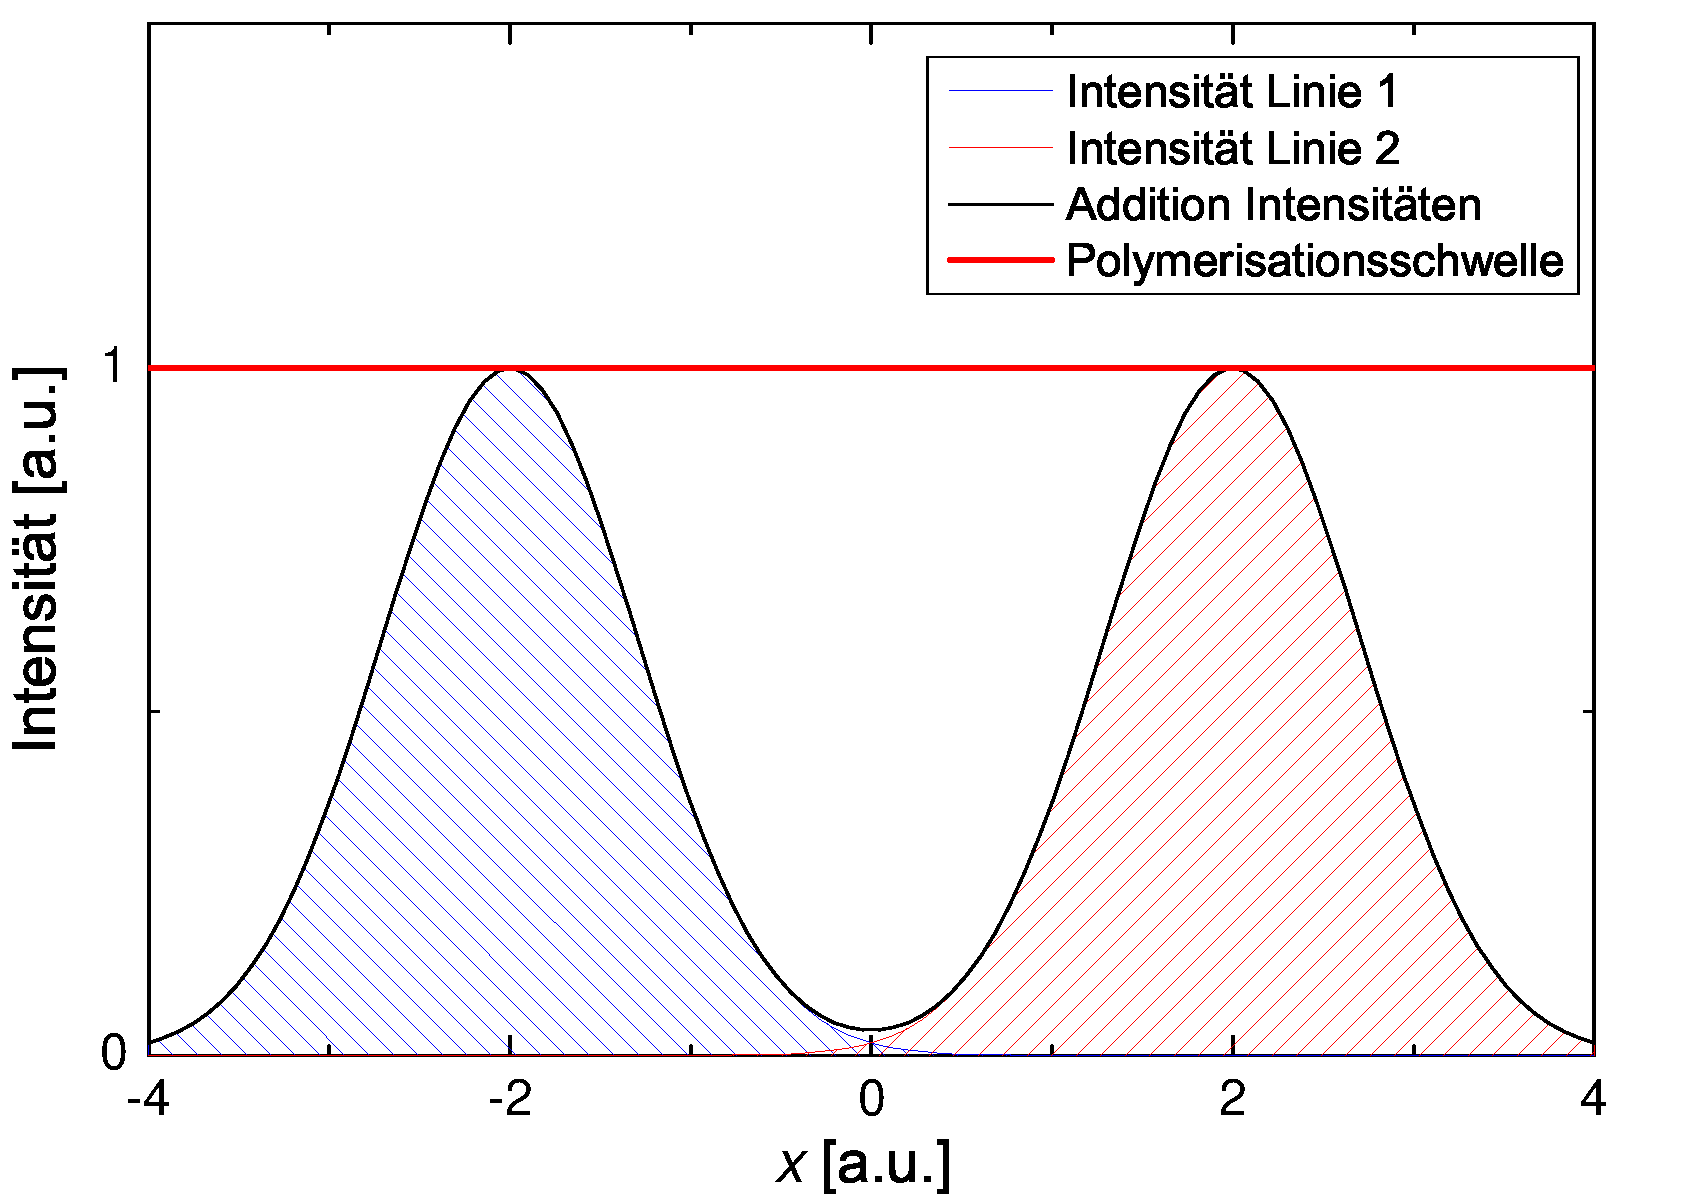
\includegraphics[totalheight=6 cm]{Grafiken/Gauss1.pdf}\label{fig:Gauss1}}
	\subfloat[]{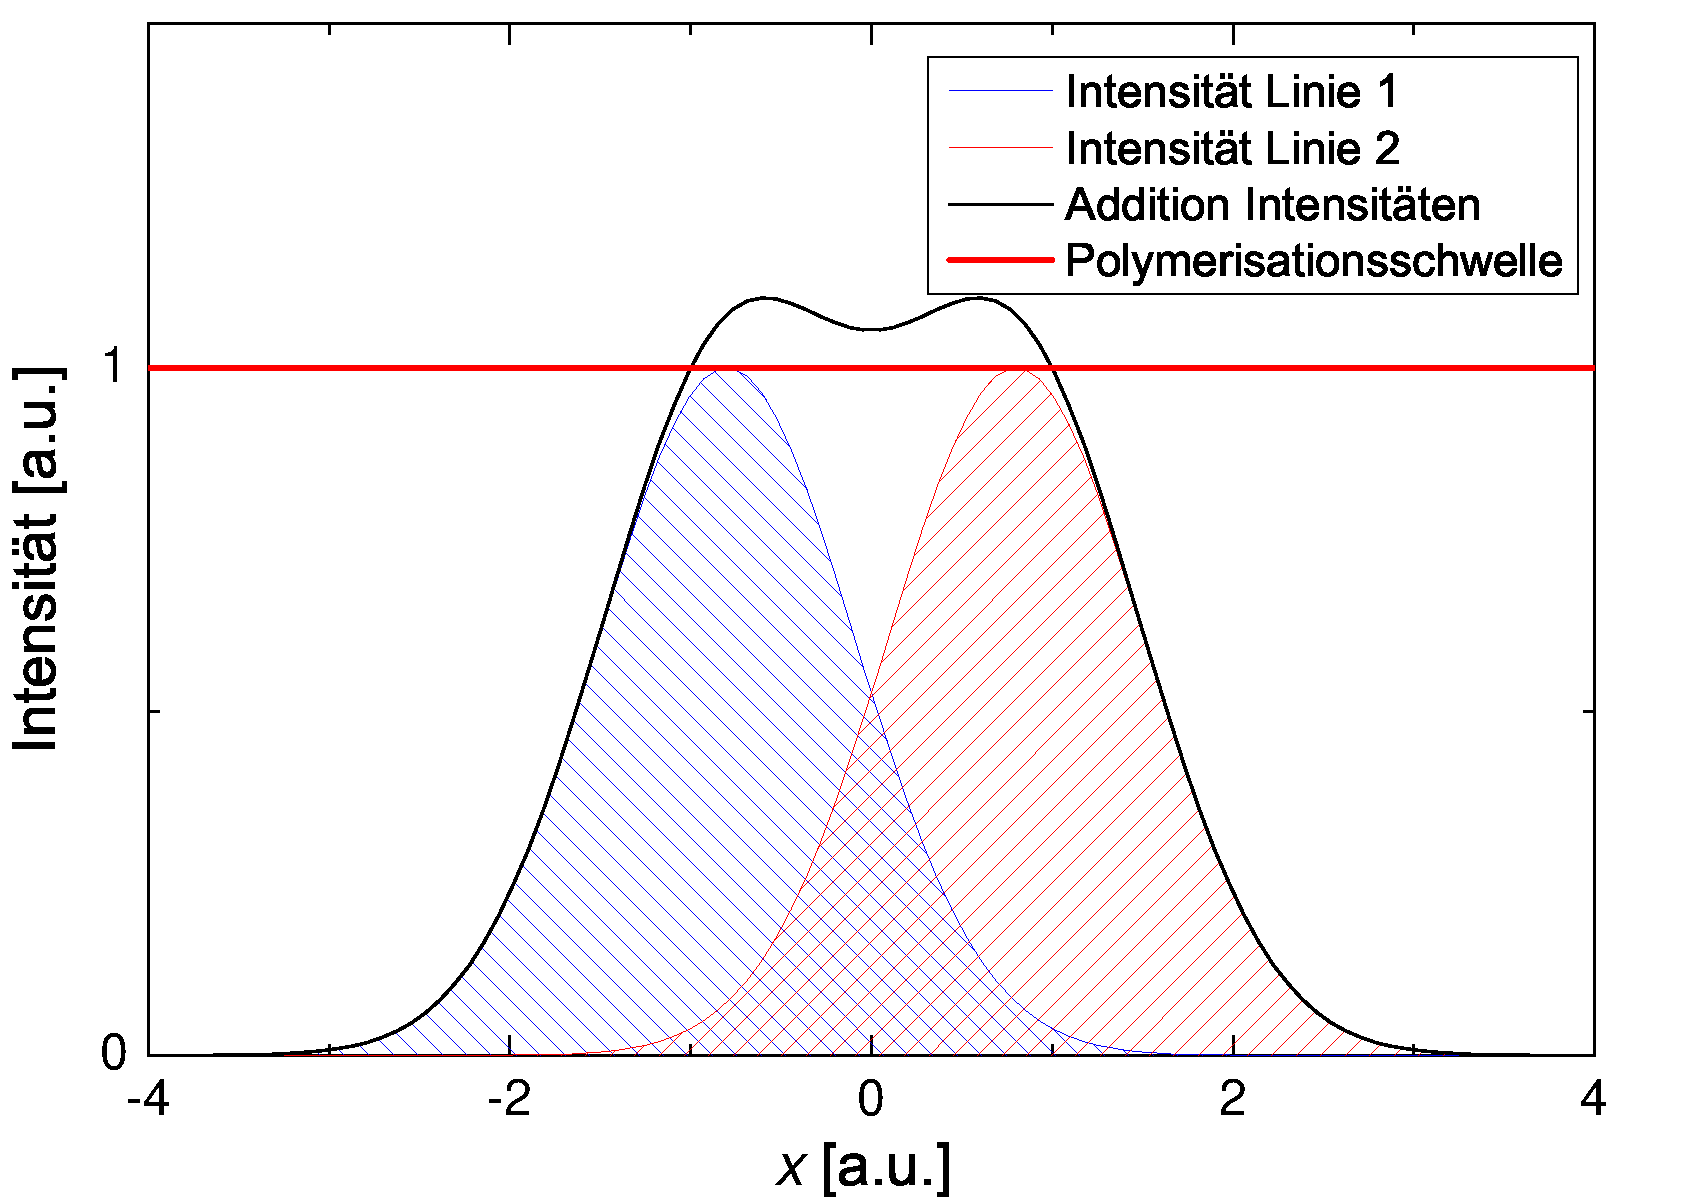
\includegraphics[totalheight=6 cm]{Grafiken/Gauss2.pdf} \label{fig:Gauss2}}%
\end{adjustwidth}
\caption{\textbf{(a)} Die Intensit�ten des Lasers reicht nicht zur Polymerisation aus. Beide Linien werden nicht geschrieben.  \textbf{(b)} Die Intensit�ten beider Linien �berlagern sich und es kommt zu einer Belichtung des Lackes.}%
\label{fig:Gauss}%
\end{figure}

Beim Betrachten von Abbildung \ref{fig:Gitter} zeigt sich, dass die einzelnen Linien der Gitterstruktur nicht vorhanden sind. Dies kann zum einen dadurch erkl�rt werden, dass beim Schreiben der Strukturen ein Gleichanteil der den gepulsten Laser �berlagerte vorhanden war. Zum anderen ist eine Unterentwicklung des Lackes denkbar, sodass die Linienzwischenr�ume nicht entwickelt wurden.


\chapter{Zusammenfassung}

Der Versuch "`Direct Laser Writing und Rasterelektronenmikroskopie"' im Rahmen des Labors Nanotechnologie am Lichttechnischen Institut (LTI) bietet einen Einblick in das Arbeiten mit einem Rasterelektronenmikroskop (REM) und die Herstellung dreidimensionaler Strukturen im Mikrometerbereich mit \textit{Direct Laser Writing} (DLW).

Um das Aufl�sungsverm�gen und die Tiefensch�rfe des REMs zu untersuchen wurden Beispielproben betrachtet. Anhand dieser Beispielproben wurden die Vorteile des REMs gegen�ber des Lichtmikroskops demonstriert. 

Das Schreiben der Strukturen erfolgte mittels DLW. Die Polymerisation des Fotolacks erfolgte �ber die zwei-Photonen-Polymerisation (2PP). Die hergestellten Strukturen wurden anschlie�end mit Hilfe eines REMs charakterisiert.

Per DLW wurden Teststrukturen geschrieben, anhand derer der Einfluss von Laserleistung und Belichtungszeit auf die Voxelgr��e untersucht wurde. Anhand der Messdaten wurde die Polymerisationsschwelle des verwendeten Fotolacks zwischen $12,5~\upmu$J$~<E_{\mathrm{Schwelle}}<15~\upmu$J bestimmt.

Zur Bestimmung der Linienaufl�sung des DLW-Prozesses sollten Gitterstrukturen hergestellt werden. Aufgrund eines Gleichanteils des Lasers konnten diese nicht korrekt abgebildet werden.
 
%Aufgrund eines Gleichanteils des Lasers konnten Strukturen zur Bestimmung der Linienaufl�sung nicht korrekt geschrieben werden. 

Zur Veranschaulichung von dreidimensionalen mit DLW geschriebenen Strukturen, wurde ein mikrometergro�es LTI-Logo hergestellt.







%
%Im Versuch "`Direct Laser Writing und Raster Elektronenmikroskopie"' im Rahmen des Labors Nanotechnologie am Lichttechnischen Institut (LTI) wurden dreidimensionale Strukturen in einer Gr��enordnung von einigen Mikrometern hergestellt und charakterisiert.


%% --------------------
%% |   Bibliography   |
%% --------------------
\cleardoublepage
\phantomsection
\addcontentsline{toc}{chapter}{\bibname}

\iflanguage{english}
{\bibliographystyle{IEEEtranSA}}	% english style
{\bibliographystyle{abbrvdin}}	% german style
												  
% Use IEEEtran for numeric references
%\bibliographystyle{IEEEtranSA})

\bibliography{thesis}
\nocite{*}


%% ----------------
%% |   Appendix   |
%% ----------------
%\cleardoublepage

%% appendix.tex
%%

%% ==============================
%\chapter{Appendix}
%\label{ch:Appendix}
%% ==============================

\appendix

\iflanguage{english}
{\addchap{Appendix}}	% english style
{\addchap{Anhang}}	% german style


\section{First Appendix Section}
		\label{Anhang-Implementierung}
		
\setcounter{figure}{0}
		
\begin{figure} [ht]
  \centering
   ein Bild
  \caption{A figure}
  \label{fig:BPMNBeispiela}
\end{figure}


\dots






\end{document}
